\batchmode
\documentclass[twoside]{book}

% Packages required by doxygen
\usepackage{fixltx2e}
\usepackage{calc}
\usepackage{doxygen}
\usepackage[export]{adjustbox} % also loads graphicx
\usepackage{graphicx}
\usepackage[utf8]{inputenc}
\usepackage{makeidx}
\usepackage{multicol}
\usepackage{multirow}
\PassOptionsToPackage{warn}{textcomp}
\usepackage{textcomp}
\usepackage[nointegrals]{wasysym}
\usepackage[table]{xcolor}

% Font selection
\usepackage[T1]{fontenc}
\usepackage[scaled=.90]{helvet}
\usepackage{courier}
\usepackage{amssymb}
\usepackage{sectsty}
\renewcommand{\familydefault}{\sfdefault}
\allsectionsfont{%
  \fontseries{bc}\selectfont%
  \color{darkgray}%
}
\renewcommand{\DoxyLabelFont}{%
  \fontseries{bc}\selectfont%
  \color{darkgray}%
}
\newcommand{\+}{\discretionary{\mbox{\scriptsize$\hookleftarrow$}}{}{}}

% Page & text layout
\usepackage{geometry}
\geometry{%
  a4paper,%
  top=2.5cm,%
  bottom=2.5cm,%
  left=2.5cm,%
  right=2.5cm%
}
\tolerance=750
\hfuzz=15pt
\hbadness=750
\setlength{\emergencystretch}{15pt}
\setlength{\parindent}{0cm}
\setlength{\parskip}{3ex plus 2ex minus 2ex}
\makeatletter
\renewcommand{\paragraph}{%
  \@startsection{paragraph}{4}{0ex}{-1.0ex}{1.0ex}{%
    \normalfont\normalsize\bfseries\SS@parafont%
  }%
}
\renewcommand{\subparagraph}{%
  \@startsection{subparagraph}{5}{0ex}{-1.0ex}{1.0ex}{%
    \normalfont\normalsize\bfseries\SS@subparafont%
  }%
}
\makeatother

% Headers & footers
\usepackage{fancyhdr}
\pagestyle{fancyplain}
\fancyhead[LE]{\fancyplain{}{\bfseries\thepage}}
\fancyhead[CE]{\fancyplain{}{}}
\fancyhead[RE]{\fancyplain{}{\bfseries\leftmark}}
\fancyhead[LO]{\fancyplain{}{\bfseries\rightmark}}
\fancyhead[CO]{\fancyplain{}{}}
\fancyhead[RO]{\fancyplain{}{\bfseries\thepage}}
\fancyfoot[LE]{\fancyplain{}{}}
\fancyfoot[CE]{\fancyplain{}{}}
\fancyfoot[RE]{\fancyplain{}{\bfseries\scriptsize Generated by Doxygen }}
\fancyfoot[LO]{\fancyplain{}{\bfseries\scriptsize Generated by Doxygen }}
\fancyfoot[CO]{\fancyplain{}{}}
\fancyfoot[RO]{\fancyplain{}{}}
\renewcommand{\footrulewidth}{0.4pt}
\renewcommand{\chaptermark}[1]{%
  \markboth{#1}{}%
}
\renewcommand{\sectionmark}[1]{%
  \markright{\thesection\ #1}%
}

% Indices & bibliography
\usepackage{natbib}
\usepackage[titles]{tocloft}
\setcounter{tocdepth}{3}
\setcounter{secnumdepth}{5}
\makeindex

% Packages requested by user
\usepackage{amsmath}

% Hyperlinks (required, but should be loaded last)
\usepackage{ifpdf}
\ifpdf
  \usepackage[pdftex,pagebackref=true]{hyperref}
\else
  \usepackage[ps2pdf,pagebackref=true]{hyperref}
\fi
\hypersetup{%
  colorlinks=true,%
  linkcolor=blue,%
  citecolor=blue,%
  unicode%
}

% Custom commands
\newcommand{\clearemptydoublepage}{%
  \newpage{\pagestyle{empty}\cleardoublepage}%
}

\usepackage{caption}
\captionsetup{labelsep=space,justification=centering,font={bf},singlelinecheck=off,skip=4pt,position=top}

%===== C O N T E N T S =====

\begin{document}

% Titlepage & ToC
\hypersetup{pageanchor=false,
             bookmarksnumbered=true
            }
\pagenumbering{alph}
\pagenumbering{arabic}
\hypersetup{pageanchor=true}

%--- Begin generated contents ---
\chapter{The adaptive solution of the equations of time-\/harmonic linear elasticity on unstructured meshes}
\label{index}\hypertarget{index}{}\hypertarget{index_q}{}\section{A few quick questions...}\label{index_q}
Since {\ttfamily oomph-\/lib} is developed as open-\/source software, any evidence that the code is being downloaded and used is very helpful for us as it helps to justify our continued work on this project.

We would therefore be extremely grateful if you could provide the information requested in the form below. Pressing the \char`\"{}submit\char`\"{} button will get you to the actual download page.

{\bfseries Note\+:} 
\begin{DoxyItemize}
\item All information will be treated as confidential. 
\item If you provide your email address and check the appropriate box we will add you to our mailing list to inform you of upgrades and bug fixes to the code. Rest assured that the mailing list is {\bfseries very low volume} -- we have better things to do than to bombard you with email. 
\item If you still feel reluctant to provide any of the information requested, feel free to enter some dummy input. The form will check that {\bfseries some} information has been entered but entering your name as \char`\"{}\+Joe Cool\char`\"{} is perfectly acceptable -- this is to discourage people from not providing the information simply because they are too lazy to type... 
\end{DoxyItemize}



 







 

 \hypertarget{index_pdf}{}\section{P\+D\+F file}\label{index_pdf}
A \href{../latex/refman.pdf}{\tt pdf version} of this document is available. \end{document}

\chapter{Namespace Index}
\section{Namespace List}
Here is a list of all namespaces with brief descriptions\+:\begin{DoxyCompactList}
\item\contentsline{section}{\hyperlink{namespaceGlobal__Physical__Variables}{Global\+\_\+\+Physical\+\_\+\+Variables} \\*Global variables that represent physical properties }{\pageref{namespaceGlobal__Physical__Variables}}{}
\item\contentsline{section}{\hyperlink{namespaceoomph}{oomph} }{\pageref{namespaceoomph}}{}
\item\contentsline{section}{\hyperlink{namespacePhysical__Variables}{Physical\+\_\+\+Variables} \\*Namespace for the solution of 2D linear shell equation }{\pageref{namespacePhysical__Variables}}{}
\end{DoxyCompactList}

\chapter{Hierarchical Index}
\section{Class Hierarchy}
This inheritance list is sorted roughly, but not completely, alphabetically\+:\begin{DoxyCompactList}
\item Problem\begin{DoxyCompactList}
\item \contentsline{section}{Unstructured\+Solid\+Problem$<$ E\+L\+E\+M\+E\+NT $>$}{\pageref{classUnstructuredSolidProblem}}{}
\end{DoxyCompactList}
\end{DoxyCompactList}

\chapter{Class Index}
\section{Class List}
Here are the classes, structs, unions and interfaces with brief descriptions\+:\begin{DoxyCompactList}
\item\contentsline{section}{\hyperlink{classPMLProblem}{P\+M\+L\+Problem$<$ E\+L\+E\+M\+E\+N\+T $>$} }{\pageref{classPMLProblem}}{}
\item\contentsline{section}{\hyperlink{classGlobalParameters_1_1TestPMLMapping}{Global\+Parameters\+::\+Test\+P\+M\+L\+Mapping} }{\pageref{classGlobalParameters_1_1TestPMLMapping}}{}
\end{DoxyCompactList}

\chapter{File Index}
\section{File List}
Here is a list of all files with brief descriptions\+:\begin{DoxyCompactList}
\item\contentsline{section}{\hyperlink{jeffery__orbit_8cc}{jeffery\+\_\+orbit.\+cc} }{\pageref{jeffery__orbit_8cc}}{}
\item\contentsline{section}{\hyperlink{jeffery__orbit_8txt__doxygenified_8h}{jeffery\+\_\+orbit.\+txt\+\_\+doxygenified.\+h} }{\pageref{jeffery__orbit_8txt__doxygenified_8h}}{}
\item\contentsline{section}{\hyperlink{my__taylor__hood__elements_8h}{my\+\_\+taylor\+\_\+hood\+\_\+elements.\+h} }{\pageref{my__taylor__hood__elements_8h}}{}
\end{DoxyCompactList}

\chapter{Namespace Documentation}
\hypertarget{namespaceGlobal__Parameters}{}\section{Global\+\_\+\+Parameters Namespace Reference}
\label{namespaceGlobal__Parameters}\index{Global\+\_\+\+Parameters@{Global\+\_\+\+Parameters}}


Global variables.  


\subsection*{Functions}
\begin{DoxyCompactItemize}
\item 
void \hyperlink{namespaceGlobal__Parameters_a200109847bf4cc26da4d00e8d68d569e}{gravity} (const double \&time, const Vector$<$ double $>$ \&xi, Vector$<$ double $>$ \&b)
\begin{DoxyCompactList}\small\item\em Non-\/dimensional gravity as body force. \end{DoxyCompactList}\item 
double \hyperlink{namespaceGlobal__Parameters_a536aa5314a6cdb36af852e9513351d55}{flux} (const double \&t)
\begin{DoxyCompactList}\small\item\em Flux increases between Min\+\_\+flux and Max\+\_\+flux over period Ramp\+\_\+period. \end{DoxyCompactList}\item 
void \hyperlink{namespaceGlobal__Parameters_a8c333f9041cad78d5c0160a8e2c169f5}{set\+\_\+parameters} (const string \&case\+\_\+id)
\begin{DoxyCompactList}\small\item\em Set parameters for the various test cases. \end{DoxyCompactList}\end{DoxyCompactItemize}
\subsection*{Variables}
\begin{DoxyCompactItemize}
\item 
string \hyperlink{namespaceGlobal__Parameters_a887474a9be53363806b4de417f660dba}{Case\+\_\+\+ID} =\char`\"{}F\+S\+I1\char`\"{}
\begin{DoxyCompactList}\small\item\em Default case ID. \end{DoxyCompactList}\item 
double \hyperlink{namespaceGlobal__Parameters_a9d72e94a9305c6a310940a6a427ebe06}{Re} =20.\+0
\begin{DoxyCompactList}\small\item\em Reynolds number (default assignment for F\+S\+I1 test case) \end{DoxyCompactList}\item 
double \hyperlink{namespaceGlobal__Parameters_af1af40a0df651e86bc1be273fafa98da}{St} =0.\+5
\begin{DoxyCompactList}\small\item\em Strouhal number (default assignment for F\+S\+I1 test case) \end{DoxyCompactList}\item 
double \hyperlink{namespaceGlobal__Parameters_a7a59a32365e87566069e458dc83bd18a}{Re\+St} =10.\+0
\begin{DoxyCompactList}\small\item\em Product of Reynolds and Strouhal numbers (default assignment for F\+S\+I1 test case) \end{DoxyCompactList}\item 
double \hyperlink{namespaceGlobal__Parameters_a7814fddf663e56168174a42d2cd6b4c1}{Q} =1.\+429e-\/6
\begin{DoxyCompactList}\small\item\em F\+SI parameter (default assignment for F\+S\+I1 test case) \end{DoxyCompactList}\item 
double \hyperlink{namespaceGlobal__Parameters_a517d4c31b8bce6563c2f605266dd9679}{Density\+\_\+ratio} =1.\+0
\begin{DoxyCompactList}\small\item\em Density ratio (solid to fluid; default assignment for F\+S\+I1 test case) \end{DoxyCompactList}\item 
double \hyperlink{namespaceGlobal__Parameters_ab360628e7830e43e355ce5768f6d6a6c}{H} =0.\+2
\begin{DoxyCompactList}\small\item\em Height of flag. \end{DoxyCompactList}\item 
double \hyperlink{namespaceGlobal__Parameters_a0f0247cc83ba202413b50e7b4b7fceb0}{Centre\+\_\+x} =2.\+0
\begin{DoxyCompactList}\small\item\em x position of centre of cylinder \end{DoxyCompactList}\item 
double \hyperlink{namespaceGlobal__Parameters_af41282d812fdff4867e3d8c825886290}{Centre\+\_\+y} =2.\+0
\begin{DoxyCompactList}\small\item\em y position of centre of cylinder \end{DoxyCompactList}\item 
double \hyperlink{namespaceGlobal__Parameters_a126c1e491ef187867b6b7bfb52b476ad}{Radius} =0.\+5
\begin{DoxyCompactList}\small\item\em Radius of cylinder. \end{DoxyCompactList}\item 
Constitutive\+Law $\ast$ \hyperlink{namespaceGlobal__Parameters_adbd1f040f375c96fe56b3f475f7dbec2}{Constitutive\+\_\+law\+\_\+pt} =0
\begin{DoxyCompactList}\small\item\em Pointer to constitutive law. \end{DoxyCompactList}\item 
double \hyperlink{namespaceGlobal__Parameters_a3e3428638f89f970fcf2148b0bab1465}{Lambda\+\_\+sq} =0.\+0
\begin{DoxyCompactList}\small\item\em Timescale ratio for solid (dependent parameter assigned in \hyperlink{namespaceGlobal__Parameters_a8c333f9041cad78d5c0160a8e2c169f5}{set\+\_\+parameters()}) \end{DoxyCompactList}\item 
double \hyperlink{namespaceGlobal__Parameters_ab29c9f716872de235c78e62bce2c4109}{Dt} =0.\+1
\begin{DoxyCompactList}\small\item\em Timestep. \end{DoxyCompactList}\item 
bool \hyperlink{namespaceGlobal__Parameters_aac13d615d2acd78d22a3137ffd62f7aa}{Ignore\+\_\+fluid\+\_\+loading} =false
\begin{DoxyCompactList}\small\item\em Ignore fluid (default assignment for F\+S\+I1 test case) \end{DoxyCompactList}\item 
double \hyperlink{namespaceGlobal__Parameters_aa3dfbdb1b2fd80d516850f66c96b6fd0}{E} =1.\+0
\begin{DoxyCompactList}\small\item\em Elastic modulus. \end{DoxyCompactList}\item 
double \hyperlink{namespaceGlobal__Parameters_a20fccdcfa2c15ad8b951b9ada3bb1661}{Nu} =0.\+4
\begin{DoxyCompactList}\small\item\em Poisson\textquotesingle{}s ratio. \end{DoxyCompactList}\item 
double \hyperlink{namespaceGlobal__Parameters_a335000b5db4206486a116ae0468d2d0c}{Gravity} =0.\+0
\begin{DoxyCompactList}\small\item\em Non-\/dim gravity (default assignment for F\+S\+I1 test case) \end{DoxyCompactList}\item 
double \hyperlink{namespaceGlobal__Parameters_af6afcca0b1ffdf88144f99cdfed18d3b}{Ramp\+\_\+period} =2.\+0
\begin{DoxyCompactList}\small\item\em Period for ramping up in flux. \end{DoxyCompactList}\item 
double \hyperlink{namespaceGlobal__Parameters_a5aabde2d31d07e5d0a84f6ff02c263dc}{Min\+\_\+flux} =0.\+0
\begin{DoxyCompactList}\small\item\em Min. flux. \end{DoxyCompactList}\item 
double \hyperlink{namespaceGlobal__Parameters_a13f0d5d16393d21bbc904aea5cff4ea4}{Max\+\_\+flux} =1.\+0
\begin{DoxyCompactList}\small\item\em Max. flux. \end{DoxyCompactList}\end{DoxyCompactItemize}


\subsection{Detailed Description}
Global variables. 

\subsection{Function Documentation}
\mbox{\Hypertarget{namespaceGlobal__Parameters_a536aa5314a6cdb36af852e9513351d55}\label{namespaceGlobal__Parameters_a536aa5314a6cdb36af852e9513351d55}} 
\index{Global\+\_\+\+Parameters@{Global\+\_\+\+Parameters}!flux@{flux}}
\index{flux@{flux}!Global\+\_\+\+Parameters@{Global\+\_\+\+Parameters}}
\subsubsection{\texorpdfstring{flux()}{flux()}}
{\footnotesize\ttfamily double Global\+\_\+\+Parameters\+::flux (\begin{DoxyParamCaption}\item[{const double \&}]{t }\end{DoxyParamCaption})}



Flux increases between Min\+\_\+flux and Max\+\_\+flux over period Ramp\+\_\+period. 



Definition at line 132 of file turek\+\_\+flag.\+cc.



References Max\+\_\+flux, and Min\+\_\+flux.



Referenced by Turek\+Problem$<$ F\+L\+U\+I\+D\+\_\+\+E\+L\+E\+M\+E\+N\+T, S\+O\+L\+I\+D\+\_\+\+E\+L\+E\+M\+E\+N\+T $>$\+::actions\+\_\+before\+\_\+implicit\+\_\+timestep(), Turek\+Problem$<$ F\+L\+U\+I\+D\+\_\+\+E\+L\+E\+M\+E\+N\+T, S\+O\+L\+I\+D\+\_\+\+E\+L\+E\+M\+E\+N\+T $>$\+::doc\+\_\+solution(), and Turek\+Problem$<$ F\+L\+U\+I\+D\+\_\+\+E\+L\+E\+M\+E\+N\+T, S\+O\+L\+I\+D\+\_\+\+E\+L\+E\+M\+E\+N\+T $>$\+::\+Turek\+Problem().

\mbox{\Hypertarget{namespaceGlobal__Parameters_a200109847bf4cc26da4d00e8d68d569e}\label{namespaceGlobal__Parameters_a200109847bf4cc26da4d00e8d68d569e}} 
\index{Global\+\_\+\+Parameters@{Global\+\_\+\+Parameters}!gravity@{gravity}}
\index{gravity@{gravity}!Global\+\_\+\+Parameters@{Global\+\_\+\+Parameters}}
\subsubsection{\texorpdfstring{gravity()}{gravity()}}
{\footnotesize\ttfamily void Global\+\_\+\+Parameters\+::gravity (\begin{DoxyParamCaption}\item[{const double \&}]{time,  }\item[{const Vector$<$ double $>$ \&}]{xi,  }\item[{Vector$<$ double $>$ \&}]{b }\end{DoxyParamCaption})}



Non-\/dimensional gravity as body force. 



Definition at line 113 of file turek\+\_\+flag.\+cc.



References Gravity.



Referenced by Turek\+Problem$<$ F\+L\+U\+I\+D\+\_\+\+E\+L\+E\+M\+E\+N\+T, S\+O\+L\+I\+D\+\_\+\+E\+L\+E\+M\+E\+N\+T $>$\+::\+Turek\+Problem().

\mbox{\Hypertarget{namespaceGlobal__Parameters_a8c333f9041cad78d5c0160a8e2c169f5}\label{namespaceGlobal__Parameters_a8c333f9041cad78d5c0160a8e2c169f5}} 
\index{Global\+\_\+\+Parameters@{Global\+\_\+\+Parameters}!set\+\_\+parameters@{set\+\_\+parameters}}
\index{set\+\_\+parameters@{set\+\_\+parameters}!Global\+\_\+\+Parameters@{Global\+\_\+\+Parameters}}
\subsubsection{\texorpdfstring{set\+\_\+parameters()}{set\_parameters()}}
{\footnotesize\ttfamily void Global\+\_\+\+Parameters\+::set\+\_\+parameters (\begin{DoxyParamCaption}\item[{const string \&}]{case\+\_\+id }\end{DoxyParamCaption})}



Set parameters for the various test cases. 



Definition at line 147 of file turek\+\_\+flag.\+cc.



References St.



Referenced by main().



\subsection{Variable Documentation}
\mbox{\Hypertarget{namespaceGlobal__Parameters_a887474a9be53363806b4de417f660dba}\label{namespaceGlobal__Parameters_a887474a9be53363806b4de417f660dba}} 
\index{Global\+\_\+\+Parameters@{Global\+\_\+\+Parameters}!Case\+\_\+\+ID@{Case\+\_\+\+ID}}
\index{Case\+\_\+\+ID@{Case\+\_\+\+ID}!Global\+\_\+\+Parameters@{Global\+\_\+\+Parameters}}
\subsubsection{\texorpdfstring{Case\+\_\+\+ID}{Case\_ID}}
{\footnotesize\ttfamily string Global\+\_\+\+Parameters\+::\+Case\+\_\+\+ID =\char`\"{}F\+S\+I1\char`\"{}}



Default case ID. 



Definition at line 59 of file turek\+\_\+flag.\+cc.



Referenced by main().

\mbox{\Hypertarget{namespaceGlobal__Parameters_a0f0247cc83ba202413b50e7b4b7fceb0}\label{namespaceGlobal__Parameters_a0f0247cc83ba202413b50e7b4b7fceb0}} 
\index{Global\+\_\+\+Parameters@{Global\+\_\+\+Parameters}!Centre\+\_\+x@{Centre\+\_\+x}}
\index{Centre\+\_\+x@{Centre\+\_\+x}!Global\+\_\+\+Parameters@{Global\+\_\+\+Parameters}}
\subsubsection{\texorpdfstring{Centre\+\_\+x}{Centre\_x}}
{\footnotesize\ttfamily double Global\+\_\+\+Parameters\+::\+Centre\+\_\+x =2.\+0}



x position of centre of cylinder 



Definition at line 82 of file turek\+\_\+flag.\+cc.



Referenced by Turek\+Problem$<$ F\+L\+U\+I\+D\+\_\+\+E\+L\+E\+M\+E\+N\+T, S\+O\+L\+I\+D\+\_\+\+E\+L\+E\+M\+E\+N\+T $>$\+::\+Turek\+Problem().

\mbox{\Hypertarget{namespaceGlobal__Parameters_af41282d812fdff4867e3d8c825886290}\label{namespaceGlobal__Parameters_af41282d812fdff4867e3d8c825886290}} 
\index{Global\+\_\+\+Parameters@{Global\+\_\+\+Parameters}!Centre\+\_\+y@{Centre\+\_\+y}}
\index{Centre\+\_\+y@{Centre\+\_\+y}!Global\+\_\+\+Parameters@{Global\+\_\+\+Parameters}}
\subsubsection{\texorpdfstring{Centre\+\_\+y}{Centre\_y}}
{\footnotesize\ttfamily double Global\+\_\+\+Parameters\+::\+Centre\+\_\+y =2.\+0}



y position of centre of cylinder 



Definition at line 85 of file turek\+\_\+flag.\+cc.



Referenced by Turek\+Problem$<$ F\+L\+U\+I\+D\+\_\+\+E\+L\+E\+M\+E\+N\+T, S\+O\+L\+I\+D\+\_\+\+E\+L\+E\+M\+E\+N\+T $>$\+::\+Turek\+Problem().

\mbox{\Hypertarget{namespaceGlobal__Parameters_adbd1f040f375c96fe56b3f475f7dbec2}\label{namespaceGlobal__Parameters_adbd1f040f375c96fe56b3f475f7dbec2}} 
\index{Global\+\_\+\+Parameters@{Global\+\_\+\+Parameters}!Constitutive\+\_\+law\+\_\+pt@{Constitutive\+\_\+law\+\_\+pt}}
\index{Constitutive\+\_\+law\+\_\+pt@{Constitutive\+\_\+law\+\_\+pt}!Global\+\_\+\+Parameters@{Global\+\_\+\+Parameters}}
\subsubsection{\texorpdfstring{Constitutive\+\_\+law\+\_\+pt}{Constitutive\_law\_pt}}
{\footnotesize\ttfamily Constitutive\+Law$\ast$ Global\+\_\+\+Parameters\+::\+Constitutive\+\_\+law\+\_\+pt =0}



Pointer to constitutive law. 



Definition at line 91 of file turek\+\_\+flag.\+cc.



Referenced by Turek\+Problem$<$ F\+L\+U\+I\+D\+\_\+\+E\+L\+E\+M\+E\+N\+T, S\+O\+L\+I\+D\+\_\+\+E\+L\+E\+M\+E\+N\+T $>$\+::\+Turek\+Problem().

\mbox{\Hypertarget{namespaceGlobal__Parameters_a517d4c31b8bce6563c2f605266dd9679}\label{namespaceGlobal__Parameters_a517d4c31b8bce6563c2f605266dd9679}} 
\index{Global\+\_\+\+Parameters@{Global\+\_\+\+Parameters}!Density\+\_\+ratio@{Density\+\_\+ratio}}
\index{Density\+\_\+ratio@{Density\+\_\+ratio}!Global\+\_\+\+Parameters@{Global\+\_\+\+Parameters}}
\subsubsection{\texorpdfstring{Density\+\_\+ratio}{Density\_ratio}}
{\footnotesize\ttfamily double Global\+\_\+\+Parameters\+::\+Density\+\_\+ratio =1.\+0}



Density ratio (solid to fluid; default assignment for F\+S\+I1 test case) 



Definition at line 76 of file turek\+\_\+flag.\+cc.

\mbox{\Hypertarget{namespaceGlobal__Parameters_ab29c9f716872de235c78e62bce2c4109}\label{namespaceGlobal__Parameters_ab29c9f716872de235c78e62bce2c4109}} 
\index{Global\+\_\+\+Parameters@{Global\+\_\+\+Parameters}!Dt@{Dt}}
\index{Dt@{Dt}!Global\+\_\+\+Parameters@{Global\+\_\+\+Parameters}}
\subsubsection{\texorpdfstring{Dt}{Dt}}
{\footnotesize\ttfamily double Global\+\_\+\+Parameters\+::\+Dt =0.\+1}



Timestep. 



Definition at line 98 of file turek\+\_\+flag.\+cc.



Referenced by main().

\mbox{\Hypertarget{namespaceGlobal__Parameters_aa3dfbdb1b2fd80d516850f66c96b6fd0}\label{namespaceGlobal__Parameters_aa3dfbdb1b2fd80d516850f66c96b6fd0}} 
\index{Global\+\_\+\+Parameters@{Global\+\_\+\+Parameters}!E@{E}}
\index{E@{E}!Global\+\_\+\+Parameters@{Global\+\_\+\+Parameters}}
\subsubsection{\texorpdfstring{E}{E}}
{\footnotesize\ttfamily double Global\+\_\+\+Parameters\+::E =1.\+0}



Elastic modulus. 



Definition at line 104 of file turek\+\_\+flag.\+cc.

\mbox{\Hypertarget{namespaceGlobal__Parameters_a335000b5db4206486a116ae0468d2d0c}\label{namespaceGlobal__Parameters_a335000b5db4206486a116ae0468d2d0c}} 
\index{Global\+\_\+\+Parameters@{Global\+\_\+\+Parameters}!Gravity@{Gravity}}
\index{Gravity@{Gravity}!Global\+\_\+\+Parameters@{Global\+\_\+\+Parameters}}
\subsubsection{\texorpdfstring{Gravity}{Gravity}}
{\footnotesize\ttfamily double Global\+\_\+\+Parameters\+::\+Gravity =0.\+0}



Non-\/dim gravity (default assignment for F\+S\+I1 test case) 



Definition at line 110 of file turek\+\_\+flag.\+cc.



Referenced by gravity().

\mbox{\Hypertarget{namespaceGlobal__Parameters_ab360628e7830e43e355ce5768f6d6a6c}\label{namespaceGlobal__Parameters_ab360628e7830e43e355ce5768f6d6a6c}} 
\index{Global\+\_\+\+Parameters@{Global\+\_\+\+Parameters}!H@{H}}
\index{H@{H}!Global\+\_\+\+Parameters@{Global\+\_\+\+Parameters}}
\subsubsection{\texorpdfstring{H}{H}}
{\footnotesize\ttfamily double Global\+\_\+\+Parameters\+::H =0.\+2}



Height of flag. 



Definition at line 79 of file turek\+\_\+flag.\+cc.



Referenced by Turek\+Problem$<$ F\+L\+U\+I\+D\+\_\+\+E\+L\+E\+M\+E\+N\+T, S\+O\+L\+I\+D\+\_\+\+E\+L\+E\+M\+E\+N\+T $>$\+::\+Turek\+Problem().

\mbox{\Hypertarget{namespaceGlobal__Parameters_aac13d615d2acd78d22a3137ffd62f7aa}\label{namespaceGlobal__Parameters_aac13d615d2acd78d22a3137ffd62f7aa}} 
\index{Global\+\_\+\+Parameters@{Global\+\_\+\+Parameters}!Ignore\+\_\+fluid\+\_\+loading@{Ignore\+\_\+fluid\+\_\+loading}}
\index{Ignore\+\_\+fluid\+\_\+loading@{Ignore\+\_\+fluid\+\_\+loading}!Global\+\_\+\+Parameters@{Global\+\_\+\+Parameters}}
\subsubsection{\texorpdfstring{Ignore\+\_\+fluid\+\_\+loading}{Ignore\_fluid\_loading}}
{\footnotesize\ttfamily bool Global\+\_\+\+Parameters\+::\+Ignore\+\_\+fluid\+\_\+loading =false}



Ignore fluid (default assignment for F\+S\+I1 test case) 



Definition at line 101 of file turek\+\_\+flag.\+cc.



Referenced by Turek\+Problem$<$ F\+L\+U\+I\+D\+\_\+\+E\+L\+E\+M\+E\+N\+T, S\+O\+L\+I\+D\+\_\+\+E\+L\+E\+M\+E\+N\+T $>$\+::actions\+\_\+after\+\_\+adapt(), and Turek\+Problem$<$ F\+L\+U\+I\+D\+\_\+\+E\+L\+E\+M\+E\+N\+T, S\+O\+L\+I\+D\+\_\+\+E\+L\+E\+M\+E\+N\+T $>$\+::\+Turek\+Problem().

\mbox{\Hypertarget{namespaceGlobal__Parameters_a3e3428638f89f970fcf2148b0bab1465}\label{namespaceGlobal__Parameters_a3e3428638f89f970fcf2148b0bab1465}} 
\index{Global\+\_\+\+Parameters@{Global\+\_\+\+Parameters}!Lambda\+\_\+sq@{Lambda\+\_\+sq}}
\index{Lambda\+\_\+sq@{Lambda\+\_\+sq}!Global\+\_\+\+Parameters@{Global\+\_\+\+Parameters}}
\subsubsection{\texorpdfstring{Lambda\+\_\+sq}{Lambda\_sq}}
{\footnotesize\ttfamily double Global\+\_\+\+Parameters\+::\+Lambda\+\_\+sq =0.\+0}



Timescale ratio for solid (dependent parameter assigned in \hyperlink{namespaceGlobal__Parameters_a8c333f9041cad78d5c0160a8e2c169f5}{set\+\_\+parameters()}) 



Definition at line 95 of file turek\+\_\+flag.\+cc.



Referenced by Turek\+Problem$<$ F\+L\+U\+I\+D\+\_\+\+E\+L\+E\+M\+E\+N\+T, S\+O\+L\+I\+D\+\_\+\+E\+L\+E\+M\+E\+N\+T $>$\+::\+Turek\+Problem().

\mbox{\Hypertarget{namespaceGlobal__Parameters_a13f0d5d16393d21bbc904aea5cff4ea4}\label{namespaceGlobal__Parameters_a13f0d5d16393d21bbc904aea5cff4ea4}} 
\index{Global\+\_\+\+Parameters@{Global\+\_\+\+Parameters}!Max\+\_\+flux@{Max\+\_\+flux}}
\index{Max\+\_\+flux@{Max\+\_\+flux}!Global\+\_\+\+Parameters@{Global\+\_\+\+Parameters}}
\subsubsection{\texorpdfstring{Max\+\_\+flux}{Max\_flux}}
{\footnotesize\ttfamily double Global\+\_\+\+Parameters\+::\+Max\+\_\+flux =1.\+0}



Max. flux. 



Definition at line 128 of file turek\+\_\+flag.\+cc.



Referenced by flux().

\mbox{\Hypertarget{namespaceGlobal__Parameters_a5aabde2d31d07e5d0a84f6ff02c263dc}\label{namespaceGlobal__Parameters_a5aabde2d31d07e5d0a84f6ff02c263dc}} 
\index{Global\+\_\+\+Parameters@{Global\+\_\+\+Parameters}!Min\+\_\+flux@{Min\+\_\+flux}}
\index{Min\+\_\+flux@{Min\+\_\+flux}!Global\+\_\+\+Parameters@{Global\+\_\+\+Parameters}}
\subsubsection{\texorpdfstring{Min\+\_\+flux}{Min\_flux}}
{\footnotesize\ttfamily double Global\+\_\+\+Parameters\+::\+Min\+\_\+flux =0.\+0}



Min. flux. 



Definition at line 125 of file turek\+\_\+flag.\+cc.



Referenced by flux().

\mbox{\Hypertarget{namespaceGlobal__Parameters_a20fccdcfa2c15ad8b951b9ada3bb1661}\label{namespaceGlobal__Parameters_a20fccdcfa2c15ad8b951b9ada3bb1661}} 
\index{Global\+\_\+\+Parameters@{Global\+\_\+\+Parameters}!Nu@{Nu}}
\index{Nu@{Nu}!Global\+\_\+\+Parameters@{Global\+\_\+\+Parameters}}
\subsubsection{\texorpdfstring{Nu}{Nu}}
{\footnotesize\ttfamily double Global\+\_\+\+Parameters\+::\+Nu =0.\+4}



Poisson\textquotesingle{}s ratio. 



Definition at line 107 of file turek\+\_\+flag.\+cc.

\mbox{\Hypertarget{namespaceGlobal__Parameters_a7814fddf663e56168174a42d2cd6b4c1}\label{namespaceGlobal__Parameters_a7814fddf663e56168174a42d2cd6b4c1}} 
\index{Global\+\_\+\+Parameters@{Global\+\_\+\+Parameters}!Q@{Q}}
\index{Q@{Q}!Global\+\_\+\+Parameters@{Global\+\_\+\+Parameters}}
\subsubsection{\texorpdfstring{Q}{Q}}
{\footnotesize\ttfamily double Global\+\_\+\+Parameters\+::Q =1.\+429e-\/6}



F\+SI parameter (default assignment for F\+S\+I1 test case) 



Definition at line 72 of file turek\+\_\+flag.\+cc.



Referenced by Turek\+Problem$<$ F\+L\+U\+I\+D\+\_\+\+E\+L\+E\+M\+E\+N\+T, S\+O\+L\+I\+D\+\_\+\+E\+L\+E\+M\+E\+N\+T $>$\+::\+Turek\+Problem().

\mbox{\Hypertarget{namespaceGlobal__Parameters_a126c1e491ef187867b6b7bfb52b476ad}\label{namespaceGlobal__Parameters_a126c1e491ef187867b6b7bfb52b476ad}} 
\index{Global\+\_\+\+Parameters@{Global\+\_\+\+Parameters}!Radius@{Radius}}
\index{Radius@{Radius}!Global\+\_\+\+Parameters@{Global\+\_\+\+Parameters}}
\subsubsection{\texorpdfstring{Radius}{Radius}}
{\footnotesize\ttfamily double Global\+\_\+\+Parameters\+::\+Radius =0.\+5}



Radius of cylinder. 



Definition at line 88 of file turek\+\_\+flag.\+cc.



Referenced by Turek\+Problem$<$ F\+L\+U\+I\+D\+\_\+\+E\+L\+E\+M\+E\+N\+T, S\+O\+L\+I\+D\+\_\+\+E\+L\+E\+M\+E\+N\+T $>$\+::\+Turek\+Problem().

\mbox{\Hypertarget{namespaceGlobal__Parameters_af6afcca0b1ffdf88144f99cdfed18d3b}\label{namespaceGlobal__Parameters_af6afcca0b1ffdf88144f99cdfed18d3b}} 
\index{Global\+\_\+\+Parameters@{Global\+\_\+\+Parameters}!Ramp\+\_\+period@{Ramp\+\_\+period}}
\index{Ramp\+\_\+period@{Ramp\+\_\+period}!Global\+\_\+\+Parameters@{Global\+\_\+\+Parameters}}
\subsubsection{\texorpdfstring{Ramp\+\_\+period}{Ramp\_period}}
{\footnotesize\ttfamily double Global\+\_\+\+Parameters\+::\+Ramp\+\_\+period =2.\+0}



Period for ramping up in flux. 



Definition at line 122 of file turek\+\_\+flag.\+cc.

\mbox{\Hypertarget{namespaceGlobal__Parameters_a9d72e94a9305c6a310940a6a427ebe06}\label{namespaceGlobal__Parameters_a9d72e94a9305c6a310940a6a427ebe06}} 
\index{Global\+\_\+\+Parameters@{Global\+\_\+\+Parameters}!Re@{Re}}
\index{Re@{Re}!Global\+\_\+\+Parameters@{Global\+\_\+\+Parameters}}
\subsubsection{\texorpdfstring{Re}{Re}}
{\footnotesize\ttfamily double Global\+\_\+\+Parameters\+::\+Re =20.\+0}



Reynolds number (default assignment for F\+S\+I1 test case) 



Definition at line 62 of file turek\+\_\+flag.\+cc.



Referenced by Turek\+Problem$<$ F\+L\+U\+I\+D\+\_\+\+E\+L\+E\+M\+E\+N\+T, S\+O\+L\+I\+D\+\_\+\+E\+L\+E\+M\+E\+N\+T $>$\+::\+Turek\+Problem().

\mbox{\Hypertarget{namespaceGlobal__Parameters_a7a59a32365e87566069e458dc83bd18a}\label{namespaceGlobal__Parameters_a7a59a32365e87566069e458dc83bd18a}} 
\index{Global\+\_\+\+Parameters@{Global\+\_\+\+Parameters}!Re\+St@{Re\+St}}
\index{Re\+St@{Re\+St}!Global\+\_\+\+Parameters@{Global\+\_\+\+Parameters}}
\subsubsection{\texorpdfstring{Re\+St}{ReSt}}
{\footnotesize\ttfamily double Global\+\_\+\+Parameters\+::\+Re\+St =10.\+0}



Product of Reynolds and Strouhal numbers (default assignment for F\+S\+I1 test case) 



Definition at line 69 of file turek\+\_\+flag.\+cc.



Referenced by Turek\+Problem$<$ F\+L\+U\+I\+D\+\_\+\+E\+L\+E\+M\+E\+N\+T, S\+O\+L\+I\+D\+\_\+\+E\+L\+E\+M\+E\+N\+T $>$\+::\+Turek\+Problem().

\mbox{\Hypertarget{namespaceGlobal__Parameters_af1af40a0df651e86bc1be273fafa98da}\label{namespaceGlobal__Parameters_af1af40a0df651e86bc1be273fafa98da}} 
\index{Global\+\_\+\+Parameters@{Global\+\_\+\+Parameters}!St@{St}}
\index{St@{St}!Global\+\_\+\+Parameters@{Global\+\_\+\+Parameters}}
\subsubsection{\texorpdfstring{St}{St}}
{\footnotesize\ttfamily double Global\+\_\+\+Parameters\+::\+St =0.\+5}



Strouhal number (default assignment for F\+S\+I1 test case) 



Definition at line 65 of file turek\+\_\+flag.\+cc.



Referenced by set\+\_\+parameters(), and Turek\+Problem$<$ F\+L\+U\+I\+D\+\_\+\+E\+L\+E\+M\+E\+N\+T, S\+O\+L\+I\+D\+\_\+\+E\+L\+E\+M\+E\+N\+T $>$\+::\+Turek\+Problem().


\chapter{Class Documentation}
\hypertarget{classAnnularDiskProblem}{}\section{Annular\+Disk\+Problem$<$ E\+L\+A\+S\+T\+I\+C\+I\+T\+Y\+\_\+\+E\+L\+E\+M\+E\+NT $>$ Class Template Reference}
\label{classAnnularDiskProblem}\index{Annular\+Disk\+Problem$<$ E\+L\+A\+S\+T\+I\+C\+I\+T\+Y\+\_\+\+E\+L\+E\+M\+E\+N\+T $>$@{Annular\+Disk\+Problem$<$ E\+L\+A\+S\+T\+I\+C\+I\+T\+Y\+\_\+\+E\+L\+E\+M\+E\+N\+T $>$}}


Annular disk.  


Inheritance diagram for Annular\+Disk\+Problem$<$ E\+L\+A\+S\+T\+I\+C\+I\+T\+Y\+\_\+\+E\+L\+E\+M\+E\+NT $>$\+:\begin{figure}[H]
\begin{center}
\leavevmode
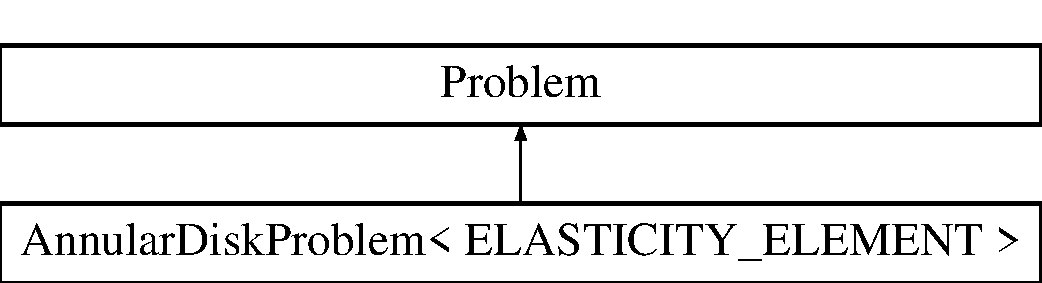
\includegraphics[height=2.000000cm]{classAnnularDiskProblem}
\end{center}
\end{figure}
\subsection*{Public Member Functions}
\begin{DoxyCompactItemize}
\item 
\hyperlink{classAnnularDiskProblem_aad1ce56fa5c26045fb14d46acf29c89e}{Annular\+Disk\+Problem} ()
\begin{DoxyCompactList}\small\item\em Constructor\+: \end{DoxyCompactList}\item 
void \hyperlink{classAnnularDiskProblem_a35d3a481c66849a57b9797c2338b8fc2}{actions\+\_\+after\+\_\+newton\+\_\+solve} ()
\begin{DoxyCompactList}\small\item\em Update function (empty) \end{DoxyCompactList}\item 
void \hyperlink{classAnnularDiskProblem_a147e5fbe37f7132bbace2b713acb03a5}{actions\+\_\+before\+\_\+newton\+\_\+solve} ()
\begin{DoxyCompactList}\small\item\em Update function (empty) \end{DoxyCompactList}\item 
void \hyperlink{classAnnularDiskProblem_a83c987045b1bdc704ed336072b8ceb16}{actions\+\_\+before\+\_\+adapt} ()
\begin{DoxyCompactList}\small\item\em Actions before adapt\+: Wipe the mesh of traction elements. \end{DoxyCompactList}\item 
void \hyperlink{classAnnularDiskProblem_a491ee3537f3b08d9a10942c4744d8d2b}{actions\+\_\+after\+\_\+adapt} ()
\begin{DoxyCompactList}\small\item\em Actions after adapt\+: Rebuild the mesh of traction elements. \end{DoxyCompactList}\item 
void \hyperlink{classAnnularDiskProblem_a8034c630f21ccf5882a21eef2c1464fc}{doc\+\_\+solution} ()
\begin{DoxyCompactList}\small\item\em Doc the solution. \end{DoxyCompactList}\end{DoxyCompactItemize}
\subsection*{Private Member Functions}
\begin{DoxyCompactItemize}
\item 
void \hyperlink{classAnnularDiskProblem_aeab547741d3b500af5f465e52e1ba57c}{create\+\_\+traction\+\_\+elements} ()
\begin{DoxyCompactList}\small\item\em Create traction elements. \end{DoxyCompactList}\item 
void \hyperlink{classAnnularDiskProblem_ae665013c94a3277cd1bf124158a4e8f2}{delete\+\_\+traction\+\_\+elements} ()
\begin{DoxyCompactList}\small\item\em Delete traction elements. \end{DoxyCompactList}\end{DoxyCompactItemize}
\subsection*{Private Attributes}
\begin{DoxyCompactItemize}
\item 
Tree\+Based\+Refineable\+Mesh\+Base $\ast$ \hyperlink{classAnnularDiskProblem_a7ef68977578d396e673a57bdf35f931c}{Solid\+\_\+mesh\+\_\+pt}
\begin{DoxyCompactList}\small\item\em Pointer to refineable solid mesh. \end{DoxyCompactList}\item 
Mesh $\ast$ \hyperlink{classAnnularDiskProblem_a2cc0ee9d7a87cdd2857b1c34e9d14c00}{Solid\+\_\+mesh\+\_\+pt}
\begin{DoxyCompactList}\small\item\em Pointer to solid mesh. \end{DoxyCompactList}\item 
Mesh $\ast$ \hyperlink{classAnnularDiskProblem_ac35f917b7678de36c2942530fc9ba4d6}{Traction\+\_\+mesh\+\_\+pt}
\begin{DoxyCompactList}\small\item\em Pointer to mesh of traction elements. \end{DoxyCompactList}\item 
Doc\+Info \hyperlink{classAnnularDiskProblem_aabdb5b1d506e3f758629c87395d0747d}{Doc\+\_\+info}
\begin{DoxyCompactList}\small\item\em Doc\+Info object for output. \end{DoxyCompactList}\end{DoxyCompactItemize}


\subsection{Detailed Description}
\subsubsection*{template$<$class E\+L\+A\+S\+T\+I\+C\+I\+T\+Y\+\_\+\+E\+L\+E\+M\+E\+NT$>$\newline
class Annular\+Disk\+Problem$<$ E\+L\+A\+S\+T\+I\+C\+I\+T\+Y\+\_\+\+E\+L\+E\+M\+E\+N\+T $>$}

Annular disk. 

Definition at line 304 of file time\+\_\+harmonic\+\_\+elastic\+\_\+annulus.\+cc.



\subsection{Constructor \& Destructor Documentation}
\mbox{\Hypertarget{classAnnularDiskProblem_aad1ce56fa5c26045fb14d46acf29c89e}\label{classAnnularDiskProblem_aad1ce56fa5c26045fb14d46acf29c89e}} 
\index{Annular\+Disk\+Problem@{Annular\+Disk\+Problem}!Annular\+Disk\+Problem@{Annular\+Disk\+Problem}}
\index{Annular\+Disk\+Problem@{Annular\+Disk\+Problem}!Annular\+Disk\+Problem@{Annular\+Disk\+Problem}}
\subsubsection{\texorpdfstring{Annular\+Disk\+Problem()}{AnnularDiskProblem()}}
{\footnotesize\ttfamily template$<$class E\+L\+A\+S\+T\+I\+C\+I\+T\+Y\+\_\+\+E\+L\+E\+M\+E\+NT $>$ \\
\hyperlink{classAnnularDiskProblem}{Annular\+Disk\+Problem}$<$ E\+L\+A\+S\+T\+I\+C\+I\+T\+Y\+\_\+\+E\+L\+E\+M\+E\+NT $>$\+::\hyperlink{classAnnularDiskProblem}{Annular\+Disk\+Problem} (\begin{DoxyParamCaption}{ }\end{DoxyParamCaption})}



Constructor\+: 



Definition at line 360 of file time\+\_\+harmonic\+\_\+elastic\+\_\+annulus.\+cc.



References Global\+\_\+\+Parameters\+::\+Directory, Global\+\_\+\+Parameters\+::\+E(), Global\+\_\+\+Parameters\+::\+H\+\_\+annulus, Global\+\_\+\+Parameters\+::\+Nr, Global\+\_\+\+Parameters\+::\+Ntheta, Global\+\_\+\+Parameters\+::\+Omega\+\_\+sq, and Global\+\_\+\+Parameters\+::solid\+\_\+boundary\+\_\+displacement().



\subsection{Member Function Documentation}
\mbox{\Hypertarget{classAnnularDiskProblem_a491ee3537f3b08d9a10942c4744d8d2b}\label{classAnnularDiskProblem_a491ee3537f3b08d9a10942c4744d8d2b}} 
\index{Annular\+Disk\+Problem@{Annular\+Disk\+Problem}!actions\+\_\+after\+\_\+adapt@{actions\+\_\+after\+\_\+adapt}}
\index{actions\+\_\+after\+\_\+adapt@{actions\+\_\+after\+\_\+adapt}!Annular\+Disk\+Problem@{Annular\+Disk\+Problem}}
\subsubsection{\texorpdfstring{actions\+\_\+after\+\_\+adapt()}{actions\_after\_adapt()}}
{\footnotesize\ttfamily template$<$class E\+L\+A\+S\+T\+I\+C\+I\+T\+Y\+\_\+\+E\+L\+E\+M\+E\+NT $>$ \\
void \hyperlink{classAnnularDiskProblem}{Annular\+Disk\+Problem}$<$ E\+L\+A\+S\+T\+I\+C\+I\+T\+Y\+\_\+\+E\+L\+E\+M\+E\+NT $>$\+::actions\+\_\+after\+\_\+adapt (\begin{DoxyParamCaption}{ }\end{DoxyParamCaption})}



Actions after adapt\+: Rebuild the mesh of traction elements. 



Definition at line 510 of file time\+\_\+harmonic\+\_\+elastic\+\_\+annulus.\+cc.

\mbox{\Hypertarget{classAnnularDiskProblem_a35d3a481c66849a57b9797c2338b8fc2}\label{classAnnularDiskProblem_a35d3a481c66849a57b9797c2338b8fc2}} 
\index{Annular\+Disk\+Problem@{Annular\+Disk\+Problem}!actions\+\_\+after\+\_\+newton\+\_\+solve@{actions\+\_\+after\+\_\+newton\+\_\+solve}}
\index{actions\+\_\+after\+\_\+newton\+\_\+solve@{actions\+\_\+after\+\_\+newton\+\_\+solve}!Annular\+Disk\+Problem@{Annular\+Disk\+Problem}}
\subsubsection{\texorpdfstring{actions\+\_\+after\+\_\+newton\+\_\+solve()}{actions\_after\_newton\_solve()}}
{\footnotesize\ttfamily template$<$class E\+L\+A\+S\+T\+I\+C\+I\+T\+Y\+\_\+\+E\+L\+E\+M\+E\+NT$>$ \\
void \hyperlink{classAnnularDiskProblem}{Annular\+Disk\+Problem}$<$ E\+L\+A\+S\+T\+I\+C\+I\+T\+Y\+\_\+\+E\+L\+E\+M\+E\+NT $>$\+::actions\+\_\+after\+\_\+newton\+\_\+solve (\begin{DoxyParamCaption}{ }\end{DoxyParamCaption})\hspace{0.3cm}{\ttfamily [inline]}}



Update function (empty) 



Definition at line 313 of file time\+\_\+harmonic\+\_\+elastic\+\_\+annulus.\+cc.

\mbox{\Hypertarget{classAnnularDiskProblem_a83c987045b1bdc704ed336072b8ceb16}\label{classAnnularDiskProblem_a83c987045b1bdc704ed336072b8ceb16}} 
\index{Annular\+Disk\+Problem@{Annular\+Disk\+Problem}!actions\+\_\+before\+\_\+adapt@{actions\+\_\+before\+\_\+adapt}}
\index{actions\+\_\+before\+\_\+adapt@{actions\+\_\+before\+\_\+adapt}!Annular\+Disk\+Problem@{Annular\+Disk\+Problem}}
\subsubsection{\texorpdfstring{actions\+\_\+before\+\_\+adapt()}{actions\_before\_adapt()}}
{\footnotesize\ttfamily template$<$class E\+L\+A\+S\+T\+I\+C\+I\+T\+Y\+\_\+\+E\+L\+E\+M\+E\+NT $>$ \\
void \hyperlink{classAnnularDiskProblem}{Annular\+Disk\+Problem}$<$ E\+L\+A\+S\+T\+I\+C\+I\+T\+Y\+\_\+\+E\+L\+E\+M\+E\+NT $>$\+::actions\+\_\+before\+\_\+adapt (\begin{DoxyParamCaption}{ }\end{DoxyParamCaption})}



Actions before adapt\+: Wipe the mesh of traction elements. 



Definition at line 494 of file time\+\_\+harmonic\+\_\+elastic\+\_\+annulus.\+cc.

\mbox{\Hypertarget{classAnnularDiskProblem_a147e5fbe37f7132bbace2b713acb03a5}\label{classAnnularDiskProblem_a147e5fbe37f7132bbace2b713acb03a5}} 
\index{Annular\+Disk\+Problem@{Annular\+Disk\+Problem}!actions\+\_\+before\+\_\+newton\+\_\+solve@{actions\+\_\+before\+\_\+newton\+\_\+solve}}
\index{actions\+\_\+before\+\_\+newton\+\_\+solve@{actions\+\_\+before\+\_\+newton\+\_\+solve}!Annular\+Disk\+Problem@{Annular\+Disk\+Problem}}
\subsubsection{\texorpdfstring{actions\+\_\+before\+\_\+newton\+\_\+solve()}{actions\_before\_newton\_solve()}}
{\footnotesize\ttfamily template$<$class E\+L\+A\+S\+T\+I\+C\+I\+T\+Y\+\_\+\+E\+L\+E\+M\+E\+NT$>$ \\
void \hyperlink{classAnnularDiskProblem}{Annular\+Disk\+Problem}$<$ E\+L\+A\+S\+T\+I\+C\+I\+T\+Y\+\_\+\+E\+L\+E\+M\+E\+NT $>$\+::actions\+\_\+before\+\_\+newton\+\_\+solve (\begin{DoxyParamCaption}{ }\end{DoxyParamCaption})\hspace{0.3cm}{\ttfamily [inline]}}



Update function (empty) 



Definition at line 316 of file time\+\_\+harmonic\+\_\+elastic\+\_\+annulus.\+cc.

\mbox{\Hypertarget{classAnnularDiskProblem_aeab547741d3b500af5f465e52e1ba57c}\label{classAnnularDiskProblem_aeab547741d3b500af5f465e52e1ba57c}} 
\index{Annular\+Disk\+Problem@{Annular\+Disk\+Problem}!create\+\_\+traction\+\_\+elements@{create\+\_\+traction\+\_\+elements}}
\index{create\+\_\+traction\+\_\+elements@{create\+\_\+traction\+\_\+elements}!Annular\+Disk\+Problem@{Annular\+Disk\+Problem}}
\subsubsection{\texorpdfstring{create\+\_\+traction\+\_\+elements()}{create\_traction\_elements()}}
{\footnotesize\ttfamily template$<$class E\+L\+A\+S\+T\+I\+C\+I\+T\+Y\+\_\+\+E\+L\+E\+M\+E\+NT $>$ \\
void \hyperlink{classAnnularDiskProblem}{Annular\+Disk\+Problem}$<$ E\+L\+A\+S\+T\+I\+C\+I\+T\+Y\+\_\+\+E\+L\+E\+M\+E\+NT $>$\+::create\+\_\+traction\+\_\+elements (\begin{DoxyParamCaption}{ }\end{DoxyParamCaption})\hspace{0.3cm}{\ttfamily [private]}}



Create traction elements. 



Definition at line 526 of file time\+\_\+harmonic\+\_\+elastic\+\_\+annulus.\+cc.



References Global\+\_\+\+Parameters\+::constant\+\_\+pressure().

\mbox{\Hypertarget{classAnnularDiskProblem_ae665013c94a3277cd1bf124158a4e8f2}\label{classAnnularDiskProblem_ae665013c94a3277cd1bf124158a4e8f2}} 
\index{Annular\+Disk\+Problem@{Annular\+Disk\+Problem}!delete\+\_\+traction\+\_\+elements@{delete\+\_\+traction\+\_\+elements}}
\index{delete\+\_\+traction\+\_\+elements@{delete\+\_\+traction\+\_\+elements}!Annular\+Disk\+Problem@{Annular\+Disk\+Problem}}
\subsubsection{\texorpdfstring{delete\+\_\+traction\+\_\+elements()}{delete\_traction\_elements()}}
{\footnotesize\ttfamily template$<$class E\+L\+A\+S\+T\+I\+C\+I\+T\+Y\+\_\+\+E\+L\+E\+M\+E\+NT $>$ \\
void \hyperlink{classAnnularDiskProblem}{Annular\+Disk\+Problem}$<$ E\+L\+A\+S\+T\+I\+C\+I\+T\+Y\+\_\+\+E\+L\+E\+M\+E\+NT $>$\+::delete\+\_\+traction\+\_\+elements (\begin{DoxyParamCaption}{ }\end{DoxyParamCaption})\hspace{0.3cm}{\ttfamily [private]}}



Delete traction elements. 

Delete traction elements and wipe the traction meshes. 

Definition at line 581 of file time\+\_\+harmonic\+\_\+elastic\+\_\+annulus.\+cc.

\mbox{\Hypertarget{classAnnularDiskProblem_a8034c630f21ccf5882a21eef2c1464fc}\label{classAnnularDiskProblem_a8034c630f21ccf5882a21eef2c1464fc}} 
\index{Annular\+Disk\+Problem@{Annular\+Disk\+Problem}!doc\+\_\+solution@{doc\+\_\+solution}}
\index{doc\+\_\+solution@{doc\+\_\+solution}!Annular\+Disk\+Problem@{Annular\+Disk\+Problem}}
\subsubsection{\texorpdfstring{doc\+\_\+solution()}{doc\_solution()}}
{\footnotesize\ttfamily template$<$class E\+L\+A\+S\+T\+I\+C\+I\+T\+Y\+\_\+\+E\+L\+E\+M\+E\+NT $>$ \\
void \hyperlink{classAnnularDiskProblem}{Annular\+Disk\+Problem}$<$ E\+L\+A\+S\+T\+I\+C\+I\+T\+Y\+\_\+\+E\+L\+E\+M\+E\+NT $>$\+::doc\+\_\+solution (\begin{DoxyParamCaption}{ }\end{DoxyParamCaption})}



Doc the solution. 



Definition at line 606 of file time\+\_\+harmonic\+\_\+elastic\+\_\+annulus.\+cc.



References Global\+\_\+\+Parameters\+::exact\+\_\+u().



Referenced by main().



\subsection{Member Data Documentation}
\mbox{\Hypertarget{classAnnularDiskProblem_aabdb5b1d506e3f758629c87395d0747d}\label{classAnnularDiskProblem_aabdb5b1d506e3f758629c87395d0747d}} 
\index{Annular\+Disk\+Problem@{Annular\+Disk\+Problem}!Doc\+\_\+info@{Doc\+\_\+info}}
\index{Doc\+\_\+info@{Doc\+\_\+info}!Annular\+Disk\+Problem@{Annular\+Disk\+Problem}}
\subsubsection{\texorpdfstring{Doc\+\_\+info}{Doc\_info}}
{\footnotesize\ttfamily template$<$class E\+L\+A\+S\+T\+I\+C\+I\+T\+Y\+\_\+\+E\+L\+E\+M\+E\+NT$>$ \\
Doc\+Info \hyperlink{classAnnularDiskProblem}{Annular\+Disk\+Problem}$<$ E\+L\+A\+S\+T\+I\+C\+I\+T\+Y\+\_\+\+E\+L\+E\+M\+E\+NT $>$\+::Doc\+\_\+info\hspace{0.3cm}{\ttfamily [private]}}



Doc\+Info object for output. 



Definition at line 351 of file time\+\_\+harmonic\+\_\+elastic\+\_\+annulus.\+cc.

\mbox{\Hypertarget{classAnnularDiskProblem_a7ef68977578d396e673a57bdf35f931c}\label{classAnnularDiskProblem_a7ef68977578d396e673a57bdf35f931c}} 
\index{Annular\+Disk\+Problem@{Annular\+Disk\+Problem}!Solid\+\_\+mesh\+\_\+pt@{Solid\+\_\+mesh\+\_\+pt}}
\index{Solid\+\_\+mesh\+\_\+pt@{Solid\+\_\+mesh\+\_\+pt}!Annular\+Disk\+Problem@{Annular\+Disk\+Problem}}
\subsubsection{\texorpdfstring{Solid\+\_\+mesh\+\_\+pt}{Solid\_mesh\_pt}\hspace{0.1cm}{\footnotesize\ttfamily [1/2]}}
{\footnotesize\ttfamily template$<$class E\+L\+A\+S\+T\+I\+C\+I\+T\+Y\+\_\+\+E\+L\+E\+M\+E\+NT$>$ \\
Tree\+Based\+Refineable\+Mesh\+Base$\ast$ \hyperlink{classAnnularDiskProblem}{Annular\+Disk\+Problem}$<$ E\+L\+A\+S\+T\+I\+C\+I\+T\+Y\+\_\+\+E\+L\+E\+M\+E\+NT $>$\+::Solid\+\_\+mesh\+\_\+pt\hspace{0.3cm}{\ttfamily [private]}}



Pointer to refineable solid mesh. 



Definition at line 338 of file time\+\_\+harmonic\+\_\+elastic\+\_\+annulus.\+cc.

\mbox{\Hypertarget{classAnnularDiskProblem_a2cc0ee9d7a87cdd2857b1c34e9d14c00}\label{classAnnularDiskProblem_a2cc0ee9d7a87cdd2857b1c34e9d14c00}} 
\index{Annular\+Disk\+Problem@{Annular\+Disk\+Problem}!Solid\+\_\+mesh\+\_\+pt@{Solid\+\_\+mesh\+\_\+pt}}
\index{Solid\+\_\+mesh\+\_\+pt@{Solid\+\_\+mesh\+\_\+pt}!Annular\+Disk\+Problem@{Annular\+Disk\+Problem}}
\subsubsection{\texorpdfstring{Solid\+\_\+mesh\+\_\+pt}{Solid\_mesh\_pt}\hspace{0.1cm}{\footnotesize\ttfamily [2/2]}}
{\footnotesize\ttfamily template$<$class E\+L\+A\+S\+T\+I\+C\+I\+T\+Y\+\_\+\+E\+L\+E\+M\+E\+NT$>$ \\
Mesh$\ast$ \hyperlink{classAnnularDiskProblem}{Annular\+Disk\+Problem}$<$ E\+L\+A\+S\+T\+I\+C\+I\+T\+Y\+\_\+\+E\+L\+E\+M\+E\+NT $>$\+::Solid\+\_\+mesh\+\_\+pt\hspace{0.3cm}{\ttfamily [private]}}



Pointer to solid mesh. 



Definition at line 343 of file time\+\_\+harmonic\+\_\+elastic\+\_\+annulus.\+cc.

\mbox{\Hypertarget{classAnnularDiskProblem_ac35f917b7678de36c2942530fc9ba4d6}\label{classAnnularDiskProblem_ac35f917b7678de36c2942530fc9ba4d6}} 
\index{Annular\+Disk\+Problem@{Annular\+Disk\+Problem}!Traction\+\_\+mesh\+\_\+pt@{Traction\+\_\+mesh\+\_\+pt}}
\index{Traction\+\_\+mesh\+\_\+pt@{Traction\+\_\+mesh\+\_\+pt}!Annular\+Disk\+Problem@{Annular\+Disk\+Problem}}
\subsubsection{\texorpdfstring{Traction\+\_\+mesh\+\_\+pt}{Traction\_mesh\_pt}}
{\footnotesize\ttfamily template$<$class E\+L\+A\+S\+T\+I\+C\+I\+T\+Y\+\_\+\+E\+L\+E\+M\+E\+NT$>$ \\
Mesh$\ast$ \hyperlink{classAnnularDiskProblem}{Annular\+Disk\+Problem}$<$ E\+L\+A\+S\+T\+I\+C\+I\+T\+Y\+\_\+\+E\+L\+E\+M\+E\+NT $>$\+::Traction\+\_\+mesh\+\_\+pt\hspace{0.3cm}{\ttfamily [private]}}



Pointer to mesh of traction elements. 



Definition at line 348 of file time\+\_\+harmonic\+\_\+elastic\+\_\+annulus.\+cc.



The documentation for this class was generated from the following file\+:\begin{DoxyCompactItemize}
\item 
\hyperlink{time__harmonic__elastic__annulus_8cc}{time\+\_\+harmonic\+\_\+elastic\+\_\+annulus.\+cc}\end{DoxyCompactItemize}

\hypertarget{classMyStraightLine}{}\section{My\+Straight\+Line Class Reference}
\label{classMyStraightLine}\index{My\+Straight\+Line@{My\+Straight\+Line}}


Straight 1D line in 2D space.  


Inheritance diagram for My\+Straight\+Line\+:\begin{figure}[H]
\begin{center}
\leavevmode
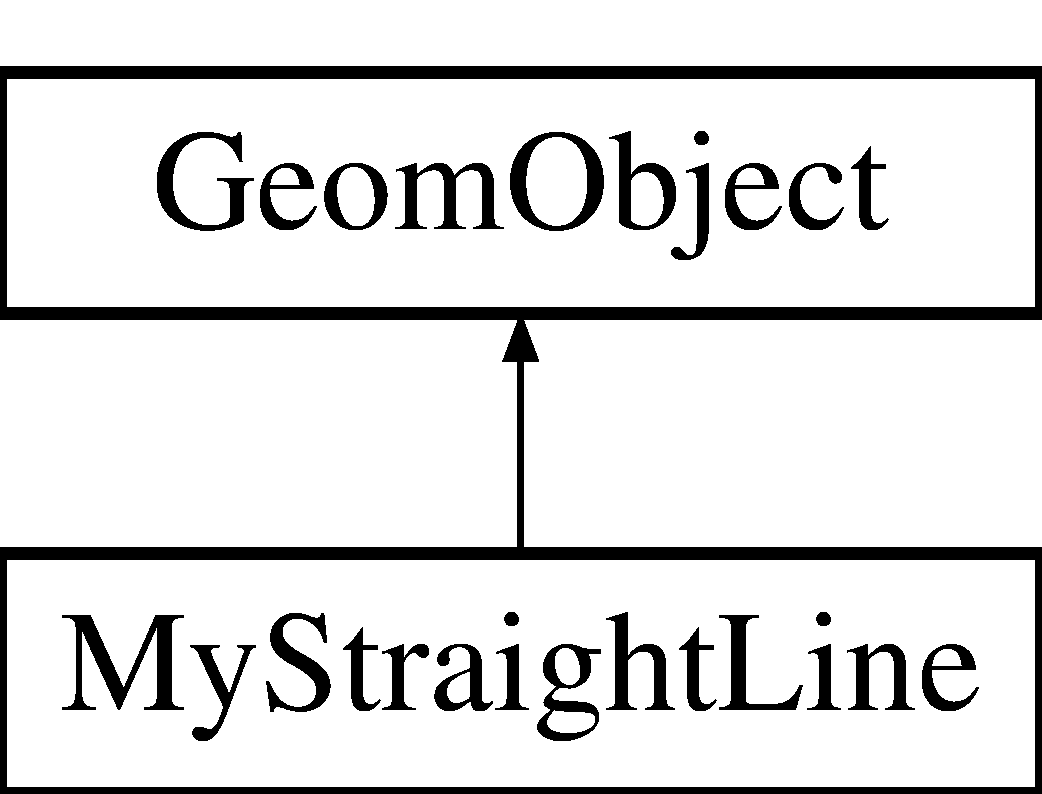
\includegraphics[height=2.000000cm]{classMyStraightLine}
\end{center}
\end{figure}
\subsection*{Public Member Functions}
\begin{DoxyCompactItemize}
\item 
\hyperlink{classMyStraightLine_a2c63e574f21703250a31fc446ab8045d}{My\+Straight\+Line} (const Vector$<$ double $>$ \&r\+\_\+start, const Vector$<$ double $>$ \&r\+\_\+end)
\begin{DoxyCompactList}\small\item\em Constructor\+: Pass start and end points. \end{DoxyCompactList}\item 
\hyperlink{classMyStraightLine_a4c42312f35a3cf72f2f39e88ad28202f}{My\+Straight\+Line} (const \hyperlink{classMyStraightLine}{My\+Straight\+Line} \&dummy)
\begin{DoxyCompactList}\small\item\em Broken copy constructor. \end{DoxyCompactList}\item 
\hyperlink{classMyStraightLine_ae2f9a5860652a726b2f4dc94d1332ef1}{$\sim$\+My\+Straight\+Line} ()
\begin{DoxyCompactList}\small\item\em Destructor\+: Empty. \end{DoxyCompactList}\item 
void \hyperlink{classMyStraightLine_ae3ee51a7b81acc2ef652bec4ee955d2f}{position} (const Vector$<$ double $>$ \&zeta, Vector$<$ double $>$ \&r) const
\begin{DoxyCompactList}\small\item\em Position Vector at Lagrangian coordinate zeta. \end{DoxyCompactList}\end{DoxyCompactItemize}
\subsection*{Private Attributes}
\begin{DoxyCompactItemize}
\item 
Vector$<$ double $>$ \hyperlink{classMyStraightLine_a0f66636dd5d1e7ff6ec93acf90879f0c}{R\+\_\+start}
\begin{DoxyCompactList}\small\item\em Start point of line. \end{DoxyCompactList}\item 
Vector$<$ double $>$ \hyperlink{classMyStraightLine_afa466e12301ccea99a02fe1bde615691}{R\+\_\+end}
\begin{DoxyCompactList}\small\item\em End point of line. \end{DoxyCompactList}\end{DoxyCompactItemize}


\subsection{Detailed Description}
Straight 1D line in 2D space. 

Definition at line 68 of file unstructured\+\_\+fourier\+\_\+decomposed\+\_\+acoustic\+\_\+fsi.\+cc.



\subsection{Constructor \& Destructor Documentation}
\mbox{\Hypertarget{classMyStraightLine_a2c63e574f21703250a31fc446ab8045d}\label{classMyStraightLine_a2c63e574f21703250a31fc446ab8045d}} 
\index{My\+Straight\+Line@{My\+Straight\+Line}!My\+Straight\+Line@{My\+Straight\+Line}}
\index{My\+Straight\+Line@{My\+Straight\+Line}!My\+Straight\+Line@{My\+Straight\+Line}}
\subsubsection{\texorpdfstring{My\+Straight\+Line()}{MyStraightLine()}\hspace{0.1cm}{\footnotesize\ttfamily [1/2]}}
{\footnotesize\ttfamily My\+Straight\+Line\+::\+My\+Straight\+Line (\begin{DoxyParamCaption}\item[{const Vector$<$ double $>$ \&}]{r\+\_\+start,  }\item[{const Vector$<$ double $>$ \&}]{r\+\_\+end }\end{DoxyParamCaption})\hspace{0.3cm}{\ttfamily [inline]}}



Constructor\+: Pass start and end points. 



Definition at line 74 of file unstructured\+\_\+fourier\+\_\+decomposed\+\_\+acoustic\+\_\+fsi.\+cc.

\mbox{\Hypertarget{classMyStraightLine_a4c42312f35a3cf72f2f39e88ad28202f}\label{classMyStraightLine_a4c42312f35a3cf72f2f39e88ad28202f}} 
\index{My\+Straight\+Line@{My\+Straight\+Line}!My\+Straight\+Line@{My\+Straight\+Line}}
\index{My\+Straight\+Line@{My\+Straight\+Line}!My\+Straight\+Line@{My\+Straight\+Line}}
\subsubsection{\texorpdfstring{My\+Straight\+Line()}{MyStraightLine()}\hspace{0.1cm}{\footnotesize\ttfamily [2/2]}}
{\footnotesize\ttfamily My\+Straight\+Line\+::\+My\+Straight\+Line (\begin{DoxyParamCaption}\item[{const \hyperlink{classMyStraightLine}{My\+Straight\+Line} \&}]{dummy }\end{DoxyParamCaption})\hspace{0.3cm}{\ttfamily [inline]}}



Broken copy constructor. 



Definition at line 80 of file unstructured\+\_\+fourier\+\_\+decomposed\+\_\+acoustic\+\_\+fsi.\+cc.

\mbox{\Hypertarget{classMyStraightLine_ae2f9a5860652a726b2f4dc94d1332ef1}\label{classMyStraightLine_ae2f9a5860652a726b2f4dc94d1332ef1}} 
\index{My\+Straight\+Line@{My\+Straight\+Line}!````~My\+Straight\+Line@{$\sim$\+My\+Straight\+Line}}
\index{````~My\+Straight\+Line@{$\sim$\+My\+Straight\+Line}!My\+Straight\+Line@{My\+Straight\+Line}}
\subsubsection{\texorpdfstring{$\sim$\+My\+Straight\+Line()}{~MyStraightLine()}}
{\footnotesize\ttfamily My\+Straight\+Line\+::$\sim$\+My\+Straight\+Line (\begin{DoxyParamCaption}{ }\end{DoxyParamCaption})\hspace{0.3cm}{\ttfamily [inline]}}



Destructor\+: Empty. 



Definition at line 86 of file unstructured\+\_\+fourier\+\_\+decomposed\+\_\+acoustic\+\_\+fsi.\+cc.



\subsection{Member Function Documentation}
\mbox{\Hypertarget{classMyStraightLine_ae3ee51a7b81acc2ef652bec4ee955d2f}\label{classMyStraightLine_ae3ee51a7b81acc2ef652bec4ee955d2f}} 
\index{My\+Straight\+Line@{My\+Straight\+Line}!position@{position}}
\index{position@{position}!My\+Straight\+Line@{My\+Straight\+Line}}
\subsubsection{\texorpdfstring{position()}{position()}}
{\footnotesize\ttfamily void My\+Straight\+Line\+::position (\begin{DoxyParamCaption}\item[{const Vector$<$ double $>$ \&}]{zeta,  }\item[{Vector$<$ double $>$ \&}]{r }\end{DoxyParamCaption}) const\hspace{0.3cm}{\ttfamily [inline]}}



Position Vector at Lagrangian coordinate zeta. 



Definition at line 89 of file unstructured\+\_\+fourier\+\_\+decomposed\+\_\+acoustic\+\_\+fsi.\+cc.



\subsection{Member Data Documentation}
\mbox{\Hypertarget{classMyStraightLine_afa466e12301ccea99a02fe1bde615691}\label{classMyStraightLine_afa466e12301ccea99a02fe1bde615691}} 
\index{My\+Straight\+Line@{My\+Straight\+Line}!R\+\_\+end@{R\+\_\+end}}
\index{R\+\_\+end@{R\+\_\+end}!My\+Straight\+Line@{My\+Straight\+Line}}
\subsubsection{\texorpdfstring{R\+\_\+end}{R\_end}}
{\footnotesize\ttfamily Vector$<$double$>$ My\+Straight\+Line\+::\+R\+\_\+end\hspace{0.3cm}{\ttfamily [private]}}



End point of line. 



Definition at line 102 of file unstructured\+\_\+fourier\+\_\+decomposed\+\_\+acoustic\+\_\+fsi.\+cc.

\mbox{\Hypertarget{classMyStraightLine_a0f66636dd5d1e7ff6ec93acf90879f0c}\label{classMyStraightLine_a0f66636dd5d1e7ff6ec93acf90879f0c}} 
\index{My\+Straight\+Line@{My\+Straight\+Line}!R\+\_\+start@{R\+\_\+start}}
\index{R\+\_\+start@{R\+\_\+start}!My\+Straight\+Line@{My\+Straight\+Line}}
\subsubsection{\texorpdfstring{R\+\_\+start}{R\_start}}
{\footnotesize\ttfamily Vector$<$double$>$ My\+Straight\+Line\+::\+R\+\_\+start\hspace{0.3cm}{\ttfamily [private]}}



Start point of line. 



Definition at line 99 of file unstructured\+\_\+fourier\+\_\+decomposed\+\_\+acoustic\+\_\+fsi.\+cc.



The documentation for this class was generated from the following file\+:\begin{DoxyCompactItemize}
\item 
\hyperlink{unstructured__fourier__decomposed__acoustic__fsi_8cc}{unstructured\+\_\+fourier\+\_\+decomposed\+\_\+acoustic\+\_\+fsi.\+cc}\end{DoxyCompactItemize}

\hypertarget{classRingWithTRibProblem}{}\section{Ring\+With\+T\+Rib\+Problem$<$ E\+L\+A\+S\+T\+I\+C\+I\+T\+Y\+\_\+\+E\+L\+E\+M\+E\+NT $>$ Class Template Reference}
\label{classRingWithTRibProblem}\index{Ring\+With\+T\+Rib\+Problem$<$ E\+L\+A\+S\+T\+I\+C\+I\+T\+Y\+\_\+\+E\+L\+E\+M\+E\+N\+T $>$@{Ring\+With\+T\+Rib\+Problem$<$ E\+L\+A\+S\+T\+I\+C\+I\+T\+Y\+\_\+\+E\+L\+E\+M\+E\+N\+T $>$}}


Annular disk.  


Inheritance diagram for Ring\+With\+T\+Rib\+Problem$<$ E\+L\+A\+S\+T\+I\+C\+I\+T\+Y\+\_\+\+E\+L\+E\+M\+E\+NT $>$\+:\begin{figure}[H]
\begin{center}
\leavevmode
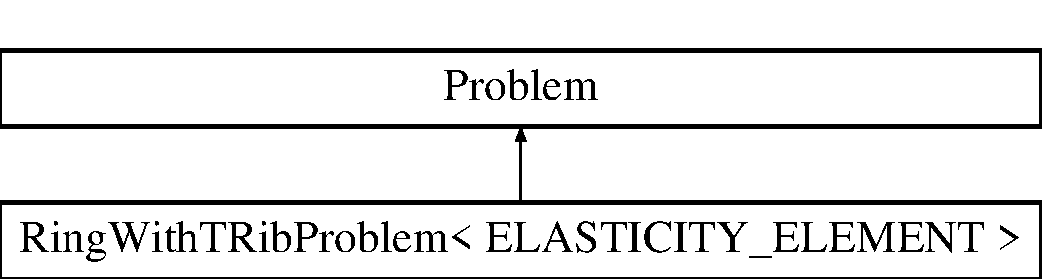
\includegraphics[height=2.000000cm]{classRingWithTRibProblem}
\end{center}
\end{figure}
\subsection*{Public Member Functions}
\begin{DoxyCompactItemize}
\item 
\hyperlink{classRingWithTRibProblem_ad0313aac3c0cdb87e753ba474a4e334f}{Ring\+With\+T\+Rib\+Problem} ()
\begin{DoxyCompactList}\small\item\em Constructor\+: \end{DoxyCompactList}\item 
void \hyperlink{classRingWithTRibProblem_a5d9f7b05cc71c02275f6c3c1a465fd20}{actions\+\_\+after\+\_\+newton\+\_\+solve} ()
\begin{DoxyCompactList}\small\item\em Update function (empty) \end{DoxyCompactList}\item 
void \hyperlink{classRingWithTRibProblem_aa74a20d5bd6d7f16eb00080734dde0d1}{actions\+\_\+before\+\_\+newton\+\_\+solve} ()
\begin{DoxyCompactList}\small\item\em Update function (empty) \end{DoxyCompactList}\item 
void \hyperlink{classRingWithTRibProblem_a7a170199d58390ae43a044294bfc7ac5}{actions\+\_\+before\+\_\+adapt} ()
\begin{DoxyCompactList}\small\item\em Actions before adapt\+: Wipe the mesh of traction elements. \end{DoxyCompactList}\item 
void \hyperlink{classRingWithTRibProblem_a8749aaf1e46d802c210b51e07093505b}{actions\+\_\+after\+\_\+adapt} ()
\begin{DoxyCompactList}\small\item\em Actions after adapt\+: Rebuild the mesh of traction elements. \end{DoxyCompactList}\item 
void \hyperlink{classRingWithTRibProblem_a43b70b125f467aa5bb9c74d08f193aa5}{doc\+\_\+solution} ()
\begin{DoxyCompactList}\small\item\em Doc the solution. \end{DoxyCompactList}\end{DoxyCompactItemize}
\subsection*{Private Member Functions}
\begin{DoxyCompactItemize}
\item 
void \hyperlink{classRingWithTRibProblem_ac4445c7a9fbfdcb69063d36fe0fe08c3}{create\+\_\+traction\+\_\+elements} ()
\begin{DoxyCompactList}\small\item\em Create traction elements. \end{DoxyCompactList}\item 
void \hyperlink{classRingWithTRibProblem_aa85169a96623cb39f18111ee436f5b9d}{delete\+\_\+traction\+\_\+elements} ()
\begin{DoxyCompactList}\small\item\em Delete traction elements. \end{DoxyCompactList}\item 
void \hyperlink{classRingWithTRibProblem_a7aa8c978ec6ff0a9823ef895b263fb41}{complete\+\_\+problem\+\_\+setup} ()
\begin{DoxyCompactList}\small\item\em Helper function to complete problem setup. \end{DoxyCompactList}\end{DoxyCompactItemize}
\subsection*{Private Attributes}
\begin{DoxyCompactItemize}
\item 
Refineable\+Triangle\+Mesh$<$ E\+L\+A\+S\+T\+I\+C\+I\+T\+Y\+\_\+\+E\+L\+E\+M\+E\+NT $>$ $\ast$ \hyperlink{classRingWithTRibProblem_a89da884cecc2d8984168817de7b1927e}{Solid\+\_\+mesh\+\_\+pt}
\begin{DoxyCompactList}\small\item\em Pointer to refineable solid mesh. \end{DoxyCompactList}\item 
Triangle\+Mesh$<$ E\+L\+A\+S\+T\+I\+C\+I\+T\+Y\+\_\+\+E\+L\+E\+M\+E\+NT $>$ $\ast$ \hyperlink{classRingWithTRibProblem_ac9502dc1955f4d3d40adb5ca581aacb6}{Solid\+\_\+mesh\+\_\+pt}
\begin{DoxyCompactList}\small\item\em Pointer to solid mesh. \end{DoxyCompactList}\item 
Mesh $\ast$ \hyperlink{classRingWithTRibProblem_abf11b5c5d0c63c91ca7b248c18acad5b}{Traction\+\_\+mesh\+\_\+pt}
\begin{DoxyCompactList}\small\item\em Pointer to mesh of traction elements. \end{DoxyCompactList}\item 
Doc\+Info \hyperlink{classRingWithTRibProblem_a086bb927e3091b5d38e193b2ccb84e3b}{Doc\+\_\+info}
\begin{DoxyCompactList}\small\item\em Doc\+Info object for output. \end{DoxyCompactList}\item 
unsigned \hyperlink{classRingWithTRibProblem_ad15da3f1436b47c6cd7a79962aaa895d}{Upper\+\_\+symmetry\+\_\+boundary\+\_\+id}
\begin{DoxyCompactList}\small\item\em Boundary ID of upper symmetry boundary. \end{DoxyCompactList}\item 
unsigned \hyperlink{classRingWithTRibProblem_a93f5abb451b85f65316b930802c727f8}{Lower\+\_\+symmetry\+\_\+boundary\+\_\+id}
\begin{DoxyCompactList}\small\item\em Boundary ID of lower symmetry boundary. \end{DoxyCompactList}\item 
unsigned \hyperlink{classRingWithTRibProblem_a88918269cac403640e2659d48210d03c}{Outer\+\_\+boundary\+\_\+id}
\begin{DoxyCompactList}\small\item\em Boundary ID of outer boundary. \end{DoxyCompactList}\end{DoxyCompactItemize}


\subsection{Detailed Description}
\subsubsection*{template$<$class E\+L\+A\+S\+T\+I\+C\+I\+T\+Y\+\_\+\+E\+L\+E\+M\+E\+NT$>$\newline
class Ring\+With\+T\+Rib\+Problem$<$ E\+L\+A\+S\+T\+I\+C\+I\+T\+Y\+\_\+\+E\+L\+E\+M\+E\+N\+T $>$}

Annular disk. 

Definition at line 159 of file unstructured\+\_\+time\+\_\+harmonic\+\_\+elastic\+\_\+annulus.\+cc.



\subsection{Constructor \& Destructor Documentation}
\mbox{\Hypertarget{classRingWithTRibProblem_ad0313aac3c0cdb87e753ba474a4e334f}\label{classRingWithTRibProblem_ad0313aac3c0cdb87e753ba474a4e334f}} 
\index{Ring\+With\+T\+Rib\+Problem@{Ring\+With\+T\+Rib\+Problem}!Ring\+With\+T\+Rib\+Problem@{Ring\+With\+T\+Rib\+Problem}}
\index{Ring\+With\+T\+Rib\+Problem@{Ring\+With\+T\+Rib\+Problem}!Ring\+With\+T\+Rib\+Problem@{Ring\+With\+T\+Rib\+Problem}}
\subsubsection{\texorpdfstring{Ring\+With\+T\+Rib\+Problem()}{RingWithTRibProblem()}}
{\footnotesize\ttfamily template$<$class E\+L\+A\+S\+T\+I\+C\+I\+T\+Y\+\_\+\+E\+L\+E\+M\+E\+NT $>$ \\
\hyperlink{classRingWithTRibProblem}{Ring\+With\+T\+Rib\+Problem}$<$ E\+L\+A\+S\+T\+I\+C\+I\+T\+Y\+\_\+\+E\+L\+E\+M\+E\+NT $>$\+::\hyperlink{classRingWithTRibProblem}{Ring\+With\+T\+Rib\+Problem} (\begin{DoxyParamCaption}{ }\end{DoxyParamCaption})}



Constructor\+: 



Definition at line 227 of file unstructured\+\_\+time\+\_\+harmonic\+\_\+elastic\+\_\+annulus.\+cc.



References Global\+\_\+\+Parameters\+::\+Directory, Global\+\_\+\+Parameters\+::\+E\+\_\+pt, Global\+\_\+\+Parameters\+::\+H\+\_\+annulus, and Global\+\_\+\+Parameters\+::\+Nu.



\subsection{Member Function Documentation}
\mbox{\Hypertarget{classRingWithTRibProblem_a8749aaf1e46d802c210b51e07093505b}\label{classRingWithTRibProblem_a8749aaf1e46d802c210b51e07093505b}} 
\index{Ring\+With\+T\+Rib\+Problem@{Ring\+With\+T\+Rib\+Problem}!actions\+\_\+after\+\_\+adapt@{actions\+\_\+after\+\_\+adapt}}
\index{actions\+\_\+after\+\_\+adapt@{actions\+\_\+after\+\_\+adapt}!Ring\+With\+T\+Rib\+Problem@{Ring\+With\+T\+Rib\+Problem}}
\subsubsection{\texorpdfstring{actions\+\_\+after\+\_\+adapt()}{actions\_after\_adapt()}}
{\footnotesize\ttfamily template$<$class E\+L\+A\+S\+T\+I\+C\+I\+T\+Y\+\_\+\+E\+L\+E\+M\+E\+NT $>$ \\
void \hyperlink{classRingWithTRibProblem}{Ring\+With\+T\+Rib\+Problem}$<$ E\+L\+A\+S\+T\+I\+C\+I\+T\+Y\+\_\+\+E\+L\+E\+M\+E\+NT $>$\+::actions\+\_\+after\+\_\+adapt (\begin{DoxyParamCaption}{ }\end{DoxyParamCaption})}



Actions after adapt\+: Rebuild the mesh of traction elements. 



Definition at line 668 of file unstructured\+\_\+time\+\_\+harmonic\+\_\+elastic\+\_\+annulus.\+cc.

\mbox{\Hypertarget{classRingWithTRibProblem_a5d9f7b05cc71c02275f6c3c1a465fd20}\label{classRingWithTRibProblem_a5d9f7b05cc71c02275f6c3c1a465fd20}} 
\index{Ring\+With\+T\+Rib\+Problem@{Ring\+With\+T\+Rib\+Problem}!actions\+\_\+after\+\_\+newton\+\_\+solve@{actions\+\_\+after\+\_\+newton\+\_\+solve}}
\index{actions\+\_\+after\+\_\+newton\+\_\+solve@{actions\+\_\+after\+\_\+newton\+\_\+solve}!Ring\+With\+T\+Rib\+Problem@{Ring\+With\+T\+Rib\+Problem}}
\subsubsection{\texorpdfstring{actions\+\_\+after\+\_\+newton\+\_\+solve()}{actions\_after\_newton\_solve()}}
{\footnotesize\ttfamily template$<$class E\+L\+A\+S\+T\+I\+C\+I\+T\+Y\+\_\+\+E\+L\+E\+M\+E\+NT$>$ \\
void \hyperlink{classRingWithTRibProblem}{Ring\+With\+T\+Rib\+Problem}$<$ E\+L\+A\+S\+T\+I\+C\+I\+T\+Y\+\_\+\+E\+L\+E\+M\+E\+NT $>$\+::actions\+\_\+after\+\_\+newton\+\_\+solve (\begin{DoxyParamCaption}{ }\end{DoxyParamCaption})\hspace{0.3cm}{\ttfamily [inline]}}



Update function (empty) 



Definition at line 168 of file unstructured\+\_\+time\+\_\+harmonic\+\_\+elastic\+\_\+annulus.\+cc.

\mbox{\Hypertarget{classRingWithTRibProblem_a7a170199d58390ae43a044294bfc7ac5}\label{classRingWithTRibProblem_a7a170199d58390ae43a044294bfc7ac5}} 
\index{Ring\+With\+T\+Rib\+Problem@{Ring\+With\+T\+Rib\+Problem}!actions\+\_\+before\+\_\+adapt@{actions\+\_\+before\+\_\+adapt}}
\index{actions\+\_\+before\+\_\+adapt@{actions\+\_\+before\+\_\+adapt}!Ring\+With\+T\+Rib\+Problem@{Ring\+With\+T\+Rib\+Problem}}
\subsubsection{\texorpdfstring{actions\+\_\+before\+\_\+adapt()}{actions\_before\_adapt()}}
{\footnotesize\ttfamily template$<$class E\+L\+A\+S\+T\+I\+C\+I\+T\+Y\+\_\+\+E\+L\+E\+M\+E\+NT $>$ \\
void \hyperlink{classRingWithTRibProblem}{Ring\+With\+T\+Rib\+Problem}$<$ E\+L\+A\+S\+T\+I\+C\+I\+T\+Y\+\_\+\+E\+L\+E\+M\+E\+NT $>$\+::actions\+\_\+before\+\_\+adapt (\begin{DoxyParamCaption}{ }\end{DoxyParamCaption})}



Actions before adapt\+: Wipe the mesh of traction elements. 



Definition at line 652 of file unstructured\+\_\+time\+\_\+harmonic\+\_\+elastic\+\_\+annulus.\+cc.

\mbox{\Hypertarget{classRingWithTRibProblem_aa74a20d5bd6d7f16eb00080734dde0d1}\label{classRingWithTRibProblem_aa74a20d5bd6d7f16eb00080734dde0d1}} 
\index{Ring\+With\+T\+Rib\+Problem@{Ring\+With\+T\+Rib\+Problem}!actions\+\_\+before\+\_\+newton\+\_\+solve@{actions\+\_\+before\+\_\+newton\+\_\+solve}}
\index{actions\+\_\+before\+\_\+newton\+\_\+solve@{actions\+\_\+before\+\_\+newton\+\_\+solve}!Ring\+With\+T\+Rib\+Problem@{Ring\+With\+T\+Rib\+Problem}}
\subsubsection{\texorpdfstring{actions\+\_\+before\+\_\+newton\+\_\+solve()}{actions\_before\_newton\_solve()}}
{\footnotesize\ttfamily template$<$class E\+L\+A\+S\+T\+I\+C\+I\+T\+Y\+\_\+\+E\+L\+E\+M\+E\+NT$>$ \\
void \hyperlink{classRingWithTRibProblem}{Ring\+With\+T\+Rib\+Problem}$<$ E\+L\+A\+S\+T\+I\+C\+I\+T\+Y\+\_\+\+E\+L\+E\+M\+E\+NT $>$\+::actions\+\_\+before\+\_\+newton\+\_\+solve (\begin{DoxyParamCaption}{ }\end{DoxyParamCaption})\hspace{0.3cm}{\ttfamily [inline]}}



Update function (empty) 



Definition at line 171 of file unstructured\+\_\+time\+\_\+harmonic\+\_\+elastic\+\_\+annulus.\+cc.

\mbox{\Hypertarget{classRingWithTRibProblem_a7aa8c978ec6ff0a9823ef895b263fb41}\label{classRingWithTRibProblem_a7aa8c978ec6ff0a9823ef895b263fb41}} 
\index{Ring\+With\+T\+Rib\+Problem@{Ring\+With\+T\+Rib\+Problem}!complete\+\_\+problem\+\_\+setup@{complete\+\_\+problem\+\_\+setup}}
\index{complete\+\_\+problem\+\_\+setup@{complete\+\_\+problem\+\_\+setup}!Ring\+With\+T\+Rib\+Problem@{Ring\+With\+T\+Rib\+Problem}}
\subsubsection{\texorpdfstring{complete\+\_\+problem\+\_\+setup()}{complete\_problem\_setup()}}
{\footnotesize\ttfamily template$<$class E\+L\+A\+S\+T\+I\+C\+I\+T\+Y\+\_\+\+E\+L\+E\+M\+E\+NT $>$ \\
void \hyperlink{classRingWithTRibProblem}{Ring\+With\+T\+Rib\+Problem}$<$ E\+L\+A\+S\+T\+I\+C\+I\+T\+Y\+\_\+\+E\+L\+E\+M\+E\+NT $>$\+::complete\+\_\+problem\+\_\+setup (\begin{DoxyParamCaption}{ }\end{DoxyParamCaption})\hspace{0.3cm}{\ttfamily [private]}}



Helper function to complete problem setup. 

Complete problem setup. 

Definition at line 570 of file unstructured\+\_\+time\+\_\+harmonic\+\_\+elastic\+\_\+annulus.\+cc.



References Global\+\_\+\+Parameters\+::\+E\+\_\+pt, and Global\+\_\+\+Parameters\+::\+Omega\+\_\+sq\+\_\+region().

\mbox{\Hypertarget{classRingWithTRibProblem_ac4445c7a9fbfdcb69063d36fe0fe08c3}\label{classRingWithTRibProblem_ac4445c7a9fbfdcb69063d36fe0fe08c3}} 
\index{Ring\+With\+T\+Rib\+Problem@{Ring\+With\+T\+Rib\+Problem}!create\+\_\+traction\+\_\+elements@{create\+\_\+traction\+\_\+elements}}
\index{create\+\_\+traction\+\_\+elements@{create\+\_\+traction\+\_\+elements}!Ring\+With\+T\+Rib\+Problem@{Ring\+With\+T\+Rib\+Problem}}
\subsubsection{\texorpdfstring{create\+\_\+traction\+\_\+elements()}{create\_traction\_elements()}}
{\footnotesize\ttfamily template$<$class E\+L\+A\+S\+T\+I\+C\+I\+T\+Y\+\_\+\+E\+L\+E\+M\+E\+NT $>$ \\
void \hyperlink{classRingWithTRibProblem}{Ring\+With\+T\+Rib\+Problem}$<$ E\+L\+A\+S\+T\+I\+C\+I\+T\+Y\+\_\+\+E\+L\+E\+M\+E\+NT $>$\+::create\+\_\+traction\+\_\+elements (\begin{DoxyParamCaption}{ }\end{DoxyParamCaption})\hspace{0.3cm}{\ttfamily [private]}}



Create traction elements. 



Definition at line 687 of file unstructured\+\_\+time\+\_\+harmonic\+\_\+elastic\+\_\+annulus.\+cc.



References Global\+\_\+\+Parameters\+::pressure\+\_\+load().

\mbox{\Hypertarget{classRingWithTRibProblem_aa85169a96623cb39f18111ee436f5b9d}\label{classRingWithTRibProblem_aa85169a96623cb39f18111ee436f5b9d}} 
\index{Ring\+With\+T\+Rib\+Problem@{Ring\+With\+T\+Rib\+Problem}!delete\+\_\+traction\+\_\+elements@{delete\+\_\+traction\+\_\+elements}}
\index{delete\+\_\+traction\+\_\+elements@{delete\+\_\+traction\+\_\+elements}!Ring\+With\+T\+Rib\+Problem@{Ring\+With\+T\+Rib\+Problem}}
\subsubsection{\texorpdfstring{delete\+\_\+traction\+\_\+elements()}{delete\_traction\_elements()}}
{\footnotesize\ttfamily template$<$class E\+L\+A\+S\+T\+I\+C\+I\+T\+Y\+\_\+\+E\+L\+E\+M\+E\+NT $>$ \\
void \hyperlink{classRingWithTRibProblem}{Ring\+With\+T\+Rib\+Problem}$<$ E\+L\+A\+S\+T\+I\+C\+I\+T\+Y\+\_\+\+E\+L\+E\+M\+E\+NT $>$\+::delete\+\_\+traction\+\_\+elements (\begin{DoxyParamCaption}{ }\end{DoxyParamCaption})\hspace{0.3cm}{\ttfamily [private]}}



Delete traction elements. 

Delete traction elements and wipe the traction meshes. 

Definition at line 732 of file unstructured\+\_\+time\+\_\+harmonic\+\_\+elastic\+\_\+annulus.\+cc.

\mbox{\Hypertarget{classRingWithTRibProblem_a43b70b125f467aa5bb9c74d08f193aa5}\label{classRingWithTRibProblem_a43b70b125f467aa5bb9c74d08f193aa5}} 
\index{Ring\+With\+T\+Rib\+Problem@{Ring\+With\+T\+Rib\+Problem}!doc\+\_\+solution@{doc\+\_\+solution}}
\index{doc\+\_\+solution@{doc\+\_\+solution}!Ring\+With\+T\+Rib\+Problem@{Ring\+With\+T\+Rib\+Problem}}
\subsubsection{\texorpdfstring{doc\+\_\+solution()}{doc\_solution()}}
{\footnotesize\ttfamily template$<$class E\+L\+A\+S\+T\+I\+C\+I\+T\+Y\+\_\+\+E\+L\+E\+M\+E\+NT $>$ \\
void \hyperlink{classRingWithTRibProblem}{Ring\+With\+T\+Rib\+Problem}$<$ E\+L\+A\+S\+T\+I\+C\+I\+T\+Y\+\_\+\+E\+L\+E\+M\+E\+NT $>$\+::doc\+\_\+solution (\begin{DoxyParamCaption}{ }\end{DoxyParamCaption})}



Doc the solution. 



Definition at line 757 of file unstructured\+\_\+time\+\_\+harmonic\+\_\+elastic\+\_\+annulus.\+cc.



Referenced by main().



\subsection{Member Data Documentation}
\mbox{\Hypertarget{classRingWithTRibProblem_a086bb927e3091b5d38e193b2ccb84e3b}\label{classRingWithTRibProblem_a086bb927e3091b5d38e193b2ccb84e3b}} 
\index{Ring\+With\+T\+Rib\+Problem@{Ring\+With\+T\+Rib\+Problem}!Doc\+\_\+info@{Doc\+\_\+info}}
\index{Doc\+\_\+info@{Doc\+\_\+info}!Ring\+With\+T\+Rib\+Problem@{Ring\+With\+T\+Rib\+Problem}}
\subsubsection{\texorpdfstring{Doc\+\_\+info}{Doc\_info}}
{\footnotesize\ttfamily template$<$class E\+L\+A\+S\+T\+I\+C\+I\+T\+Y\+\_\+\+E\+L\+E\+M\+E\+NT$>$ \\
Doc\+Info \hyperlink{classRingWithTRibProblem}{Ring\+With\+T\+Rib\+Problem}$<$ E\+L\+A\+S\+T\+I\+C\+I\+T\+Y\+\_\+\+E\+L\+E\+M\+E\+NT $>$\+::Doc\+\_\+info\hspace{0.3cm}{\ttfamily [private]}}



Doc\+Info object for output. 



Definition at line 209 of file unstructured\+\_\+time\+\_\+harmonic\+\_\+elastic\+\_\+annulus.\+cc.

\mbox{\Hypertarget{classRingWithTRibProblem_a93f5abb451b85f65316b930802c727f8}\label{classRingWithTRibProblem_a93f5abb451b85f65316b930802c727f8}} 
\index{Ring\+With\+T\+Rib\+Problem@{Ring\+With\+T\+Rib\+Problem}!Lower\+\_\+symmetry\+\_\+boundary\+\_\+id@{Lower\+\_\+symmetry\+\_\+boundary\+\_\+id}}
\index{Lower\+\_\+symmetry\+\_\+boundary\+\_\+id@{Lower\+\_\+symmetry\+\_\+boundary\+\_\+id}!Ring\+With\+T\+Rib\+Problem@{Ring\+With\+T\+Rib\+Problem}}
\subsubsection{\texorpdfstring{Lower\+\_\+symmetry\+\_\+boundary\+\_\+id}{Lower\_symmetry\_boundary\_id}}
{\footnotesize\ttfamily template$<$class E\+L\+A\+S\+T\+I\+C\+I\+T\+Y\+\_\+\+E\+L\+E\+M\+E\+NT$>$ \\
unsigned \hyperlink{classRingWithTRibProblem}{Ring\+With\+T\+Rib\+Problem}$<$ E\+L\+A\+S\+T\+I\+C\+I\+T\+Y\+\_\+\+E\+L\+E\+M\+E\+NT $>$\+::Lower\+\_\+symmetry\+\_\+boundary\+\_\+id\hspace{0.3cm}{\ttfamily [private]}}



Boundary ID of lower symmetry boundary. 



Definition at line 215 of file unstructured\+\_\+time\+\_\+harmonic\+\_\+elastic\+\_\+annulus.\+cc.

\mbox{\Hypertarget{classRingWithTRibProblem_a88918269cac403640e2659d48210d03c}\label{classRingWithTRibProblem_a88918269cac403640e2659d48210d03c}} 
\index{Ring\+With\+T\+Rib\+Problem@{Ring\+With\+T\+Rib\+Problem}!Outer\+\_\+boundary\+\_\+id@{Outer\+\_\+boundary\+\_\+id}}
\index{Outer\+\_\+boundary\+\_\+id@{Outer\+\_\+boundary\+\_\+id}!Ring\+With\+T\+Rib\+Problem@{Ring\+With\+T\+Rib\+Problem}}
\subsubsection{\texorpdfstring{Outer\+\_\+boundary\+\_\+id}{Outer\_boundary\_id}}
{\footnotesize\ttfamily template$<$class E\+L\+A\+S\+T\+I\+C\+I\+T\+Y\+\_\+\+E\+L\+E\+M\+E\+NT$>$ \\
unsigned \hyperlink{classRingWithTRibProblem}{Ring\+With\+T\+Rib\+Problem}$<$ E\+L\+A\+S\+T\+I\+C\+I\+T\+Y\+\_\+\+E\+L\+E\+M\+E\+NT $>$\+::Outer\+\_\+boundary\+\_\+id\hspace{0.3cm}{\ttfamily [private]}}



Boundary ID of outer boundary. 



Definition at line 218 of file unstructured\+\_\+time\+\_\+harmonic\+\_\+elastic\+\_\+annulus.\+cc.

\mbox{\Hypertarget{classRingWithTRibProblem_a89da884cecc2d8984168817de7b1927e}\label{classRingWithTRibProblem_a89da884cecc2d8984168817de7b1927e}} 
\index{Ring\+With\+T\+Rib\+Problem@{Ring\+With\+T\+Rib\+Problem}!Solid\+\_\+mesh\+\_\+pt@{Solid\+\_\+mesh\+\_\+pt}}
\index{Solid\+\_\+mesh\+\_\+pt@{Solid\+\_\+mesh\+\_\+pt}!Ring\+With\+T\+Rib\+Problem@{Ring\+With\+T\+Rib\+Problem}}
\subsubsection{\texorpdfstring{Solid\+\_\+mesh\+\_\+pt}{Solid\_mesh\_pt}\hspace{0.1cm}{\footnotesize\ttfamily [1/2]}}
{\footnotesize\ttfamily template$<$class E\+L\+A\+S\+T\+I\+C\+I\+T\+Y\+\_\+\+E\+L\+E\+M\+E\+NT$>$ \\
Refineable\+Triangle\+Mesh$<$E\+L\+A\+S\+T\+I\+C\+I\+T\+Y\+\_\+\+E\+L\+E\+M\+E\+NT$>$$\ast$ \hyperlink{classRingWithTRibProblem}{Ring\+With\+T\+Rib\+Problem}$<$ E\+L\+A\+S\+T\+I\+C\+I\+T\+Y\+\_\+\+E\+L\+E\+M\+E\+NT $>$\+::Solid\+\_\+mesh\+\_\+pt\hspace{0.3cm}{\ttfamily [private]}}



Pointer to refineable solid mesh. 



Definition at line 196 of file unstructured\+\_\+time\+\_\+harmonic\+\_\+elastic\+\_\+annulus.\+cc.

\mbox{\Hypertarget{classRingWithTRibProblem_ac9502dc1955f4d3d40adb5ca581aacb6}\label{classRingWithTRibProblem_ac9502dc1955f4d3d40adb5ca581aacb6}} 
\index{Ring\+With\+T\+Rib\+Problem@{Ring\+With\+T\+Rib\+Problem}!Solid\+\_\+mesh\+\_\+pt@{Solid\+\_\+mesh\+\_\+pt}}
\index{Solid\+\_\+mesh\+\_\+pt@{Solid\+\_\+mesh\+\_\+pt}!Ring\+With\+T\+Rib\+Problem@{Ring\+With\+T\+Rib\+Problem}}
\subsubsection{\texorpdfstring{Solid\+\_\+mesh\+\_\+pt}{Solid\_mesh\_pt}\hspace{0.1cm}{\footnotesize\ttfamily [2/2]}}
{\footnotesize\ttfamily template$<$class E\+L\+A\+S\+T\+I\+C\+I\+T\+Y\+\_\+\+E\+L\+E\+M\+E\+NT$>$ \\
Triangle\+Mesh$<$E\+L\+A\+S\+T\+I\+C\+I\+T\+Y\+\_\+\+E\+L\+E\+M\+E\+NT$>$$\ast$ \hyperlink{classRingWithTRibProblem}{Ring\+With\+T\+Rib\+Problem}$<$ E\+L\+A\+S\+T\+I\+C\+I\+T\+Y\+\_\+\+E\+L\+E\+M\+E\+NT $>$\+::Solid\+\_\+mesh\+\_\+pt\hspace{0.3cm}{\ttfamily [private]}}



Pointer to solid mesh. 



Definition at line 201 of file unstructured\+\_\+time\+\_\+harmonic\+\_\+elastic\+\_\+annulus.\+cc.

\mbox{\Hypertarget{classRingWithTRibProblem_abf11b5c5d0c63c91ca7b248c18acad5b}\label{classRingWithTRibProblem_abf11b5c5d0c63c91ca7b248c18acad5b}} 
\index{Ring\+With\+T\+Rib\+Problem@{Ring\+With\+T\+Rib\+Problem}!Traction\+\_\+mesh\+\_\+pt@{Traction\+\_\+mesh\+\_\+pt}}
\index{Traction\+\_\+mesh\+\_\+pt@{Traction\+\_\+mesh\+\_\+pt}!Ring\+With\+T\+Rib\+Problem@{Ring\+With\+T\+Rib\+Problem}}
\subsubsection{\texorpdfstring{Traction\+\_\+mesh\+\_\+pt}{Traction\_mesh\_pt}}
{\footnotesize\ttfamily template$<$class E\+L\+A\+S\+T\+I\+C\+I\+T\+Y\+\_\+\+E\+L\+E\+M\+E\+NT$>$ \\
Mesh$\ast$ \hyperlink{classRingWithTRibProblem}{Ring\+With\+T\+Rib\+Problem}$<$ E\+L\+A\+S\+T\+I\+C\+I\+T\+Y\+\_\+\+E\+L\+E\+M\+E\+NT $>$\+::Traction\+\_\+mesh\+\_\+pt\hspace{0.3cm}{\ttfamily [private]}}



Pointer to mesh of traction elements. 



Definition at line 206 of file unstructured\+\_\+time\+\_\+harmonic\+\_\+elastic\+\_\+annulus.\+cc.

\mbox{\Hypertarget{classRingWithTRibProblem_ad15da3f1436b47c6cd7a79962aaa895d}\label{classRingWithTRibProblem_ad15da3f1436b47c6cd7a79962aaa895d}} 
\index{Ring\+With\+T\+Rib\+Problem@{Ring\+With\+T\+Rib\+Problem}!Upper\+\_\+symmetry\+\_\+boundary\+\_\+id@{Upper\+\_\+symmetry\+\_\+boundary\+\_\+id}}
\index{Upper\+\_\+symmetry\+\_\+boundary\+\_\+id@{Upper\+\_\+symmetry\+\_\+boundary\+\_\+id}!Ring\+With\+T\+Rib\+Problem@{Ring\+With\+T\+Rib\+Problem}}
\subsubsection{\texorpdfstring{Upper\+\_\+symmetry\+\_\+boundary\+\_\+id}{Upper\_symmetry\_boundary\_id}}
{\footnotesize\ttfamily template$<$class E\+L\+A\+S\+T\+I\+C\+I\+T\+Y\+\_\+\+E\+L\+E\+M\+E\+NT$>$ \\
unsigned \hyperlink{classRingWithTRibProblem}{Ring\+With\+T\+Rib\+Problem}$<$ E\+L\+A\+S\+T\+I\+C\+I\+T\+Y\+\_\+\+E\+L\+E\+M\+E\+NT $>$\+::Upper\+\_\+symmetry\+\_\+boundary\+\_\+id\hspace{0.3cm}{\ttfamily [private]}}



Boundary ID of upper symmetry boundary. 



Definition at line 212 of file unstructured\+\_\+time\+\_\+harmonic\+\_\+elastic\+\_\+annulus.\+cc.



The documentation for this class was generated from the following file\+:\begin{DoxyCompactItemize}
\item 
\hyperlink{unstructured__time__harmonic__elastic__annulus_8cc}{unstructured\+\_\+time\+\_\+harmonic\+\_\+elastic\+\_\+annulus.\+cc}\end{DoxyCompactItemize}

\chapter{File Documentation}
\hypertarget{time__harmonic__elastic__annulus_8cc}{}\section{time\+\_\+harmonic\+\_\+elastic\+\_\+annulus.\+cc File Reference}
\label{time__harmonic__elastic__annulus_8cc}\index{time\+\_\+harmonic\+\_\+elastic\+\_\+annulus.\+cc@{time\+\_\+harmonic\+\_\+elastic\+\_\+annulus.\+cc}}
\subsection*{Classes}
\begin{DoxyCompactItemize}
\item 
class \hyperlink{classAnnularDiskProblem}{Annular\+Disk\+Problem$<$ E\+L\+A\+S\+T\+I\+C\+I\+T\+Y\+\_\+\+E\+L\+E\+M\+E\+N\+T $>$}
\begin{DoxyCompactList}\small\item\em Annular disk. \end{DoxyCompactList}\end{DoxyCompactItemize}
\subsection*{Namespaces}
\begin{DoxyCompactItemize}
\item 
 \hyperlink{namespaceGlobal__Parameters}{Global\+\_\+\+Parameters}
\begin{DoxyCompactList}\small\item\em Global variables. \end{DoxyCompactList}\end{DoxyCompactItemize}
\subsection*{Functions}
\begin{DoxyCompactItemize}
\item 
Time\+Harmonic\+Isotropic\+Elasticity\+Tensor \hyperlink{namespaceGlobal__Parameters_aeeb26e11ef275bdfce14710e00290bb6}{Global\+\_\+\+Parameters\+::E} (Nu)
\begin{DoxyCompactList}\small\item\em The elasticity tensor. \end{DoxyCompactList}\item 
void \hyperlink{namespaceGlobal__Parameters_a95af753fa152ac6013bc4f640816f7ce}{Global\+\_\+\+Parameters\+::solid\+\_\+boundary\+\_\+displacement} (const Vector$<$ double $>$ \&x, Vector$<$ double $>$ \&u)
\begin{DoxyCompactList}\small\item\em Real-\/valued, radial displacement field on inner boundary. \end{DoxyCompactList}\item 
void \hyperlink{namespaceGlobal__Parameters_a8363ab9f8687e9f7802f801f6dcab6e6}{Global\+\_\+\+Parameters\+::constant\+\_\+pressure} (const Vector$<$ double $>$ \&x, const Vector$<$ double $>$ \&n, Vector$<$ std\+::complex$<$ double $>$ $>$ \&traction)
\begin{DoxyCompactList}\small\item\em Constant pressure load (real and imag part) \end{DoxyCompactList}\item 
double \hyperlink{namespaceGlobal__Parameters_a51c78ffbd213fe1293eef5d048abcc5a}{Global\+\_\+\+Parameters\+::\+BesselY} (const double \&n, const double \&x)
\begin{DoxyCompactList}\small\item\em Helper function to evaluate Y\+\_\+n(x) from bloody maple output. \end{DoxyCompactList}\item 
double \hyperlink{namespaceGlobal__Parameters_aa3dda8c7600df01ddcd31b966230c5ba}{Global\+\_\+\+Parameters\+::\+BesselJ} (const double \&n, const double \&x)
\begin{DoxyCompactList}\small\item\em Helper function to evaluate J\+\_\+n(x) from bloody maple output. \end{DoxyCompactList}\item 
void \hyperlink{namespaceGlobal__Parameters_a97162dba4bd29a15067b9c9bbe53c754}{Global\+\_\+\+Parameters\+::exact\+\_\+u} (const Vector$<$ double $>$ \&x, Vector$<$ double $>$ \&u)
\begin{DoxyCompactList}\small\item\em Exact solution as a Vector. \end{DoxyCompactList}\item 
int \hyperlink{time__harmonic__elastic__annulus_8cc_a3c04138a5bfe5d72780bb7e82a18e627}{main} (int argc, char $\ast$$\ast$argv)
\begin{DoxyCompactList}\small\item\em Driver for annular disk loaded by pressure. \end{DoxyCompactList}\end{DoxyCompactItemize}
\subsection*{Variables}
\begin{DoxyCompactItemize}
\item 
double \hyperlink{namespaceGlobal__Parameters_a20fccdcfa2c15ad8b951b9ada3bb1661}{Global\+\_\+\+Parameters\+::\+Nu} = 0.\+3
\begin{DoxyCompactList}\small\item\em Poisson\textquotesingle{}s ratio. \end{DoxyCompactList}\item 
double \hyperlink{namespaceGlobal__Parameters_af9e1e178dfb7f5e35b452599bd4c4324}{Global\+\_\+\+Parameters\+::\+Omega\+\_\+sq} =100.\+0
\begin{DoxyCompactList}\small\item\em Square of non-\/dim frequency. \end{DoxyCompactList}\item 
double \hyperlink{namespaceGlobal__Parameters_a0b73c5ead1114ae88bbd4cb0eb54f078}{Global\+\_\+\+Parameters\+::\+H\+\_\+annulus} =0.\+5
\begin{DoxyCompactList}\small\item\em Thickness of annulus. \end{DoxyCompactList}\item 
double \hyperlink{namespaceGlobal__Parameters_a0138eb659958d7d7d1afd12577becf82}{Global\+\_\+\+Parameters\+::\+Displacement\+\_\+amplitude} =0.\+1
\begin{DoxyCompactList}\small\item\em Displacement amplitude on inner radius. \end{DoxyCompactList}\item 
double \hyperlink{namespaceGlobal__Parameters_a31fb55c20db4aa0127aafa20f0d76731}{Global\+\_\+\+Parameters\+::P} = 0.\+0
\begin{DoxyCompactList}\small\item\em Uniform pressure. \end{DoxyCompactList}\item 
string \hyperlink{namespaceGlobal__Parameters_a301ab922df72030c660b21328d6caf76}{Global\+\_\+\+Parameters\+::\+Directory} =\char`\"{}R\+E\+S\+LT\char`\"{}
\begin{DoxyCompactList}\small\item\em Output directory. \end{DoxyCompactList}\item 
unsigned \hyperlink{namespaceGlobal__Parameters_a1f67286edeb13ef67687fd483e105b5e}{Global\+\_\+\+Parameters\+::\+Ntheta} =20
\begin{DoxyCompactList}\small\item\em Number of elements in azimuthal direction. \end{DoxyCompactList}\item 
unsigned \hyperlink{namespaceGlobal__Parameters_aeebb1e39d849d32cebdc9be13026606e}{Global\+\_\+\+Parameters\+::\+Nr} =10
\begin{DoxyCompactList}\small\item\em Number of elements in radial direction. \end{DoxyCompactList}\end{DoxyCompactItemize}


\subsection{Function Documentation}
\mbox{\Hypertarget{time__harmonic__elastic__annulus_8cc_a3c04138a5bfe5d72780bb7e82a18e627}\label{time__harmonic__elastic__annulus_8cc_a3c04138a5bfe5d72780bb7e82a18e627}} 
\index{time\+\_\+harmonic\+\_\+elastic\+\_\+annulus.\+cc@{time\+\_\+harmonic\+\_\+elastic\+\_\+annulus.\+cc}!main@{main}}
\index{main@{main}!time\+\_\+harmonic\+\_\+elastic\+\_\+annulus.\+cc@{time\+\_\+harmonic\+\_\+elastic\+\_\+annulus.\+cc}}
\subsubsection{\texorpdfstring{main()}{main()}}
{\footnotesize\ttfamily int main (\begin{DoxyParamCaption}\item[{int}]{argc,  }\item[{char $\ast$$\ast$}]{argv }\end{DoxyParamCaption})}



Driver for annular disk loaded by pressure. 



Definition at line 650 of file time\+\_\+harmonic\+\_\+elastic\+\_\+annulus.\+cc.



References Annular\+Disk\+Problem$<$ E\+L\+A\+S\+T\+I\+C\+I\+T\+Y\+\_\+\+E\+L\+E\+M\+E\+N\+T $>$\+::doc\+\_\+solution(), Global\+\_\+\+Parameters\+::\+Nr, Global\+\_\+\+Parameters\+::\+Ntheta, and Global\+\_\+\+Parameters\+::P.


\hypertarget{unstructured__elastic__annulus_8txt__doxygenified_8h}{}\section{unstructured\+\_\+elastic\+\_\+annulus.\+txt\+\_\+doxygenified.\+h File Reference}
\label{unstructured__elastic__annulus_8txt__doxygenified_8h}\index{unstructured\+\_\+elastic\+\_\+annulus.\+txt\+\_\+doxygenified.\+h@{unstructured\+\_\+elastic\+\_\+annulus.\+txt\+\_\+doxygenified.\+h}}

\hypertarget{unstructured__time__harmonic__elastic__annulus_8cc}{}\section{unstructured\+\_\+time\+\_\+harmonic\+\_\+elastic\+\_\+annulus.\+cc File Reference}
\label{unstructured__time__harmonic__elastic__annulus_8cc}\index{unstructured\+\_\+time\+\_\+harmonic\+\_\+elastic\+\_\+annulus.\+cc@{unstructured\+\_\+time\+\_\+harmonic\+\_\+elastic\+\_\+annulus.\+cc}}
\subsection*{Classes}
\begin{DoxyCompactItemize}
\item 
class \hyperlink{classMyStraightLine}{My\+Straight\+Line}
\begin{DoxyCompactList}\small\item\em Straight 1D line in 2D space. \end{DoxyCompactList}\item 
class \hyperlink{classRingWithTRibProblem}{Ring\+With\+T\+Rib\+Problem$<$ E\+L\+A\+S\+T\+I\+C\+I\+T\+Y\+\_\+\+E\+L\+E\+M\+E\+N\+T $>$}
\begin{DoxyCompactList}\small\item\em Annular disk. \end{DoxyCompactList}\end{DoxyCompactItemize}
\subsection*{Namespaces}
\begin{DoxyCompactItemize}
\item 
 \hyperlink{namespaceGlobal__Parameters}{Global\+\_\+\+Parameters}
\begin{DoxyCompactList}\small\item\em Global variables. \end{DoxyCompactList}\end{DoxyCompactItemize}
\subsection*{Functions}
\begin{DoxyCompactItemize}
\item 
Vector$<$ double $>$ \hyperlink{namespaceGlobal__Parameters_a58a76124a7c047adf58388cc12e84f23}{Global\+\_\+\+Parameters\+::\+Omega\+\_\+sq\+\_\+region} (2, Omega\+\_\+sq)
\begin{DoxyCompactList}\small\item\em Square of non-\/dim frequency for the two regions. \end{DoxyCompactList}\item 
void \hyperlink{namespaceGlobal__Parameters_a0ddb3a77481b907fbb34f2e8d0a6eb9f}{Global\+\_\+\+Parameters\+::pressure\+\_\+load} (const Vector$<$ double $>$ \&x, const Vector$<$ double $>$ \&n, Vector$<$ std\+::complex$<$ double $>$ $>$ \&traction)
\begin{DoxyCompactList}\small\item\em Constant pressure load (real and imag part) \end{DoxyCompactList}\item 
int \hyperlink{unstructured__time__harmonic__elastic__annulus_8cc_a3c04138a5bfe5d72780bb7e82a18e627}{main} (int argc, char $\ast$$\ast$argv)
\begin{DoxyCompactList}\small\item\em Driver for annular disk loaded by pressure. \end{DoxyCompactList}\end{DoxyCompactItemize}
\subsection*{Variables}
\begin{DoxyCompactItemize}
\item 
Vector$<$ Time\+Harmonic\+Isotropic\+Elasticity\+Tensor $\ast$ $>$ \hyperlink{namespaceGlobal__Parameters_a73c731fa617a9d92851e4195493262e7}{Global\+\_\+\+Parameters\+::\+E\+\_\+pt}
\begin{DoxyCompactList}\small\item\em The elasticity tensors for the two regions. \end{DoxyCompactList}\item 
double \hyperlink{namespaceGlobal__Parameters_afbe27ad463a1fb23cb99d029a9fac731}{Global\+\_\+\+Parameters\+::\+Alpha} =200.\+0
\begin{DoxyCompactList}\small\item\em Peakiness parameter for pressure load. \end{DoxyCompactList}\end{DoxyCompactItemize}


\subsection{Function Documentation}
\mbox{\Hypertarget{unstructured__time__harmonic__elastic__annulus_8cc_a3c04138a5bfe5d72780bb7e82a18e627}\label{unstructured__time__harmonic__elastic__annulus_8cc_a3c04138a5bfe5d72780bb7e82a18e627}} 
\index{unstructured\+\_\+time\+\_\+harmonic\+\_\+elastic\+\_\+annulus.\+cc@{unstructured\+\_\+time\+\_\+harmonic\+\_\+elastic\+\_\+annulus.\+cc}!main@{main}}
\index{main@{main}!unstructured\+\_\+time\+\_\+harmonic\+\_\+elastic\+\_\+annulus.\+cc@{unstructured\+\_\+time\+\_\+harmonic\+\_\+elastic\+\_\+annulus.\+cc}}
\subsubsection{\texorpdfstring{main()}{main()}}
{\footnotesize\ttfamily int main (\begin{DoxyParamCaption}\item[{int}]{argc,  }\item[{char $\ast$$\ast$}]{argv }\end{DoxyParamCaption})}



Driver for annular disk loaded by pressure. 



Definition at line 824 of file unstructured\+\_\+time\+\_\+harmonic\+\_\+elastic\+\_\+annulus.\+cc.



References Global\+\_\+\+Parameters\+::\+Alpha, Ring\+With\+T\+Rib\+Problem$<$ E\+L\+A\+S\+T\+I\+C\+I\+T\+Y\+\_\+\+E\+L\+E\+M\+E\+N\+T $>$\+::doc\+\_\+solution(), Global\+\_\+\+Parameters\+::\+E\+\_\+pt, Global\+\_\+\+Parameters\+::\+Nu, Global\+\_\+\+Parameters\+::\+Omega\+\_\+sq\+\_\+region(), and Global\+\_\+\+Parameters\+::P.


%--- End generated contents ---

% Index
\backmatter
\newpage
\phantomsection
\clearemptydoublepage
\addcontentsline{toc}{chapter}{Index}
\printindex

